\documentclass{article}
\usepackage{fancyhdr}
\usepackage{ctex}
\usepackage{listings}
\usepackage{graphicx}
\usepackage[a4paper, body={18cm,22cm}]{geometry}
\usepackage{amsmath,amssymb,amstext,wasysym,enumerate,graphicx}
\usepackage{float,abstract,booktabs,indentfirst,amsmath}
\usepackage{array}
\usepackage{booktabs}
\usepackage{multirow}
\usepackage{url}
\usepackage{diagbox}
\renewcommand\arraystretch{1.4}
\usepackage{indentfirst}
\setlength{\parindent}{2em}
\usepackage{enumitem}
\setmonofont{Consolas}
\usepackage{listings}
\usepackage{xcolor}
\usepackage{makecell}
\usepackage{tikz}
\usetikzlibrary{positioning, arrows.meta}
\setCJKmonofont{黑体}
\lstset{  
	% 基本设置  
	xleftmargin = 3em, xrightmargin = 3em, aboveskip = 1em,  
	backgroundcolor = \color{white},  
	basicstyle = \small\ttfamily,  
	rulesepcolor = \color{gray},  
	breaklines = true,  
	numbers = left,  
	numberstyle = \small,  
	numbersep = -14pt,  
	frame = shadowbox,  
	showspaces = false,  
	columns = fixed,  
	sensitive = true,  
	% VSCode 风格配色  
	keywordstyle = \color{blue!70!black}\bfseries,  
	emphstyle = \color{red!70!black}\bfseries, % 对于强调的词  
	emphstyle=[2]\color{purple!70!black}\bfseries, % 对于第二组强调的词  
	commentstyle = \color{green!60!black}, % 注释颜色  
	stringstyle = \color{orange!90!black}, % 字符串颜色更亮一些  
	morekeywords={ASSERT, int64\_t, uint32\_t},  
	moreemph={ASSERT, NULL},  
	moreemph=[2]{int64\_t, uint32\_t, tid\_t, uint8\_t, int16\_t, uint16\_t, int32\_t, size\_t, bool},  
	morecomment=[l][\color{green!60!black}]{+}, % 以+开头的注释  
}

%--------------------页眉--------------------%
\pagestyle{fancy}
\fancyhead[L]{}
\fancyhead[R]{}
\fancyhead[C]{华东师范大学软件工程学院实验报告}
\fancyfoot[C]{-\thepage-}
\renewcommand{\headrulewidth}{1.5pt}
%--------------------标题--------------------%
\begin{document}
\begin{center}
  {\Large{\textbf{\heiti 华东师范大学软件工程学院实验报告}}}
  \begin{table}[H]
    \centering
    \begin{tabular}{p{2cm}p{4cm}<{\centering}p{1cm}p{2cm}p{6cm}<{\centering}}
      课程名称:    & 操作系统实践 & \quad & 指导教师:    & 张民
      \\ \cline{2-2} \cline{5-5}
      姓\qquad 名: & 王海生    & \quad & 学\qquad 号: & 10235101559         \\ \cline{2-2} \cline{5-5}
      实验编号:    & 实验一 & \quad & 实验名称:    & PintOS安装
      \\ \cline{2-2} \cline{5-5}
    \end{tabular}
  \end{table}
\end{center}
\rule{\textwidth}{1pt}
%--------------------正文--------------------%
\section{实验目的}

\begin{enumerate}[noitemsep, label={{\arabic*})}]
  \item 配置PintOS运行环境
  \item 熟悉Linux常用命令
  \item 通过虚拟机、Docker等软件熟悉操作系统中的基本概念
  \item 体会不同形式的Linux之间的异同
\end{enumerate}
\normalsize
\section{实验内容与设计思想}
在本实验中,我将配置好PintOS的运行环境。由于我对操作系统有极大的兴趣,同时在学习过程中不断有同学与我讨论环境配置相关的问题,我将依次通过以下四种方式安装PintOS,并分析比较他们的优势和不足:

\begin{enumerate}[noitemsep, label={{\arabic*})}]
  \item 在运行Windows系统的x86架构计算机上,使用Virtualbox虚拟机直接导入Ubuntu系统镜像,直接运行PintOS
  \item 在运行macOS系统的ARM架构计算机上,使用Docker拉取Ubuntu系统镜像,安装并运行PintOS
  \item 在运行Windows系统的x86计算机上,使用WSL (Windows Subsystem for Linux) 安装并运行PintOS
  \item 在运行Ubuntu系统的x86服务器上,原生安装并运行PintOS
\end{enumerate}

四种方法的优势和不足如下表所示:\\

\begin{center}
\begin{tabular}{| >{\centering\arraybackslash}m{1cm} | >{\centering\arraybackslash}m{2cm} | >{\centering\arraybackslash}m{6.5cm} | >{\centering\arraybackslash}m{6.5cm} |}  
	\hline  
	\textbf{序号} & \textbf{安装方法} & \textbf{优势} & \textbf{不足} \\  
	\hline  
	1 & Virtualbox & 一键导入,最简单的方法 & GUI卡顿,常有黑屏bug \\  
	\hline  
	2 & Docker & 资源开销比虚拟机小,理论上运行更流畅,是虚拟机之外的新选择 & 国内拉取镜像缓慢;文件管理困难,需要不断创建新镜像,容易丢失修改内容 \\  
	\hline
	3 & Server & 原生Linux系统,最强性能和兼容性 & 搭建服务器需要额外的成本 \\  
	\hline
	4 & WSL & 安装较简便,资源开销介于虚拟机和Docker之间;文件管理方便 & Linux内核为修改版本,有潜在不兼容的可能;只适用于较新的Windows电脑 \\  
	\hline  

\end{tabular}
\end{center}

\section{使用环境}

\subsection{Virtualbox虚拟机}

Virtualbox主机系统环境如下表所示:

\begin{center}
	\begin{tabular}{| >{\centering\arraybackslash}m{3cm} | >{\centering\arraybackslash}m{9cm} |}    
		\hline  
		\textbf{项目名称} & \textbf{详细信息} \\
		\hline  
		操作系统 & Windows 11 专业版 23H2 \\  
		\hline  
		系统类型 & 64位操作系统,基于x64的处理器 \\  
		\hline
		CPU & 12th Gen Intel(R) Core(TM) i7-12800HX 2.00 GHz \\  
		\hline 
		GPU & NVIDIA GeForce RTX 3080 Ti Laptop (16GB)\\  
		\hline 
		内存 & 32GB DDR5 4800MHz \\  
		\hline 
		磁盘 & 1TB SSD \\  
		\hline 		
	\end{tabular}
\end{center}

在官网下载并安装后,Virtualbox虚拟机正常运行,如下图所示:

\begin{figure}[H]
  \centering
  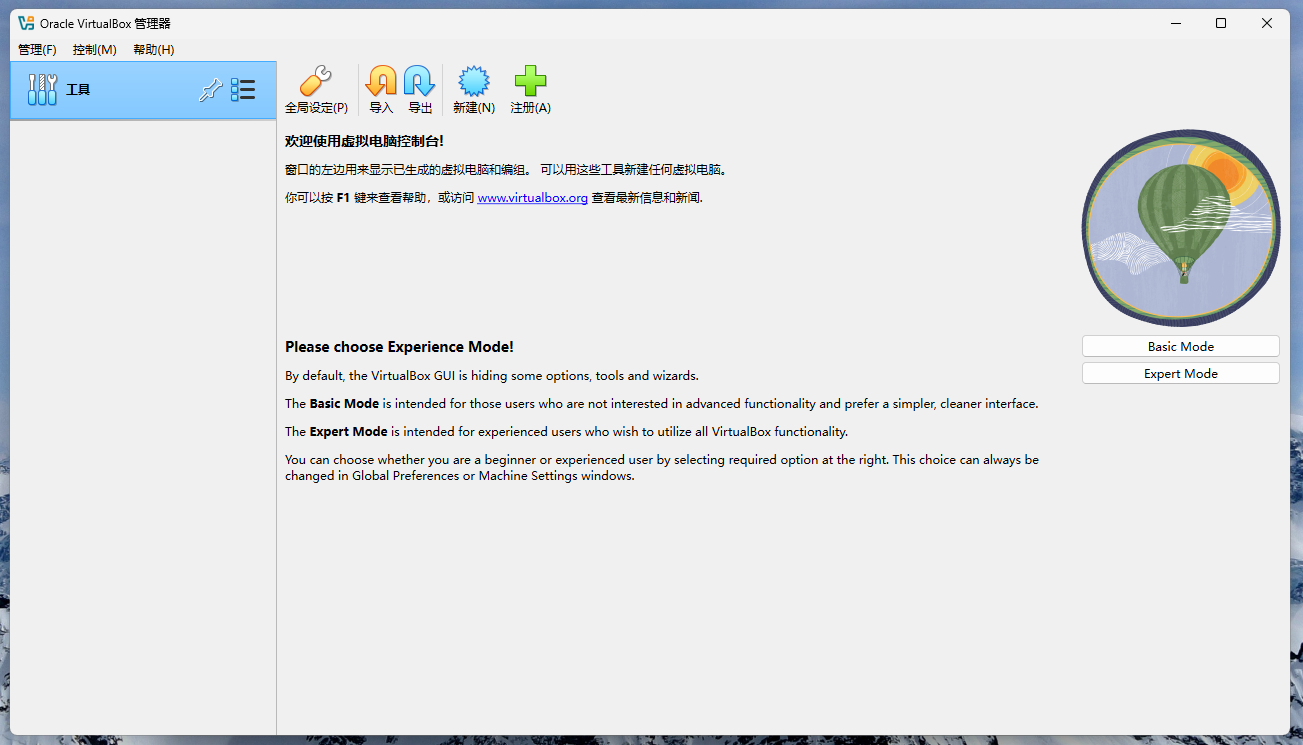
\includegraphics[width=0.9\textwidth]{img/virtual_install.png}
  \caption{Virtualbox虚拟机}
\end{figure}

\subsection{Docker容器}

Docker容器主机系统环境如下表所示:

\begin{center}
	\begin{tabular}{| >{\centering\arraybackslash}m{3cm} | >{\centering\arraybackslash}m{7cm} |}    
		\hline  
		\textbf{项目名称} & \textbf{详细信息} \\
		\hline  
		操作系统 & macOS Sequoia 15.0 \\  
		\hline  
		系统类型 & 64位操作系统,基于ARM的处理器 \\  
		\hline
		CPU & Apple M1 Pro \\  
		\hline 
		GPU & Apple M1 Pro\\  
		\hline 
		内存 & 16GB 统一内存 \\  
		\hline 
		磁盘 & 512GB SSD \\  
		\hline 		
	\end{tabular}
\end{center}

在官网下载并安装后,Docker容器正常运行,如下图所示:

\begin{figure}[H]
	\centering
	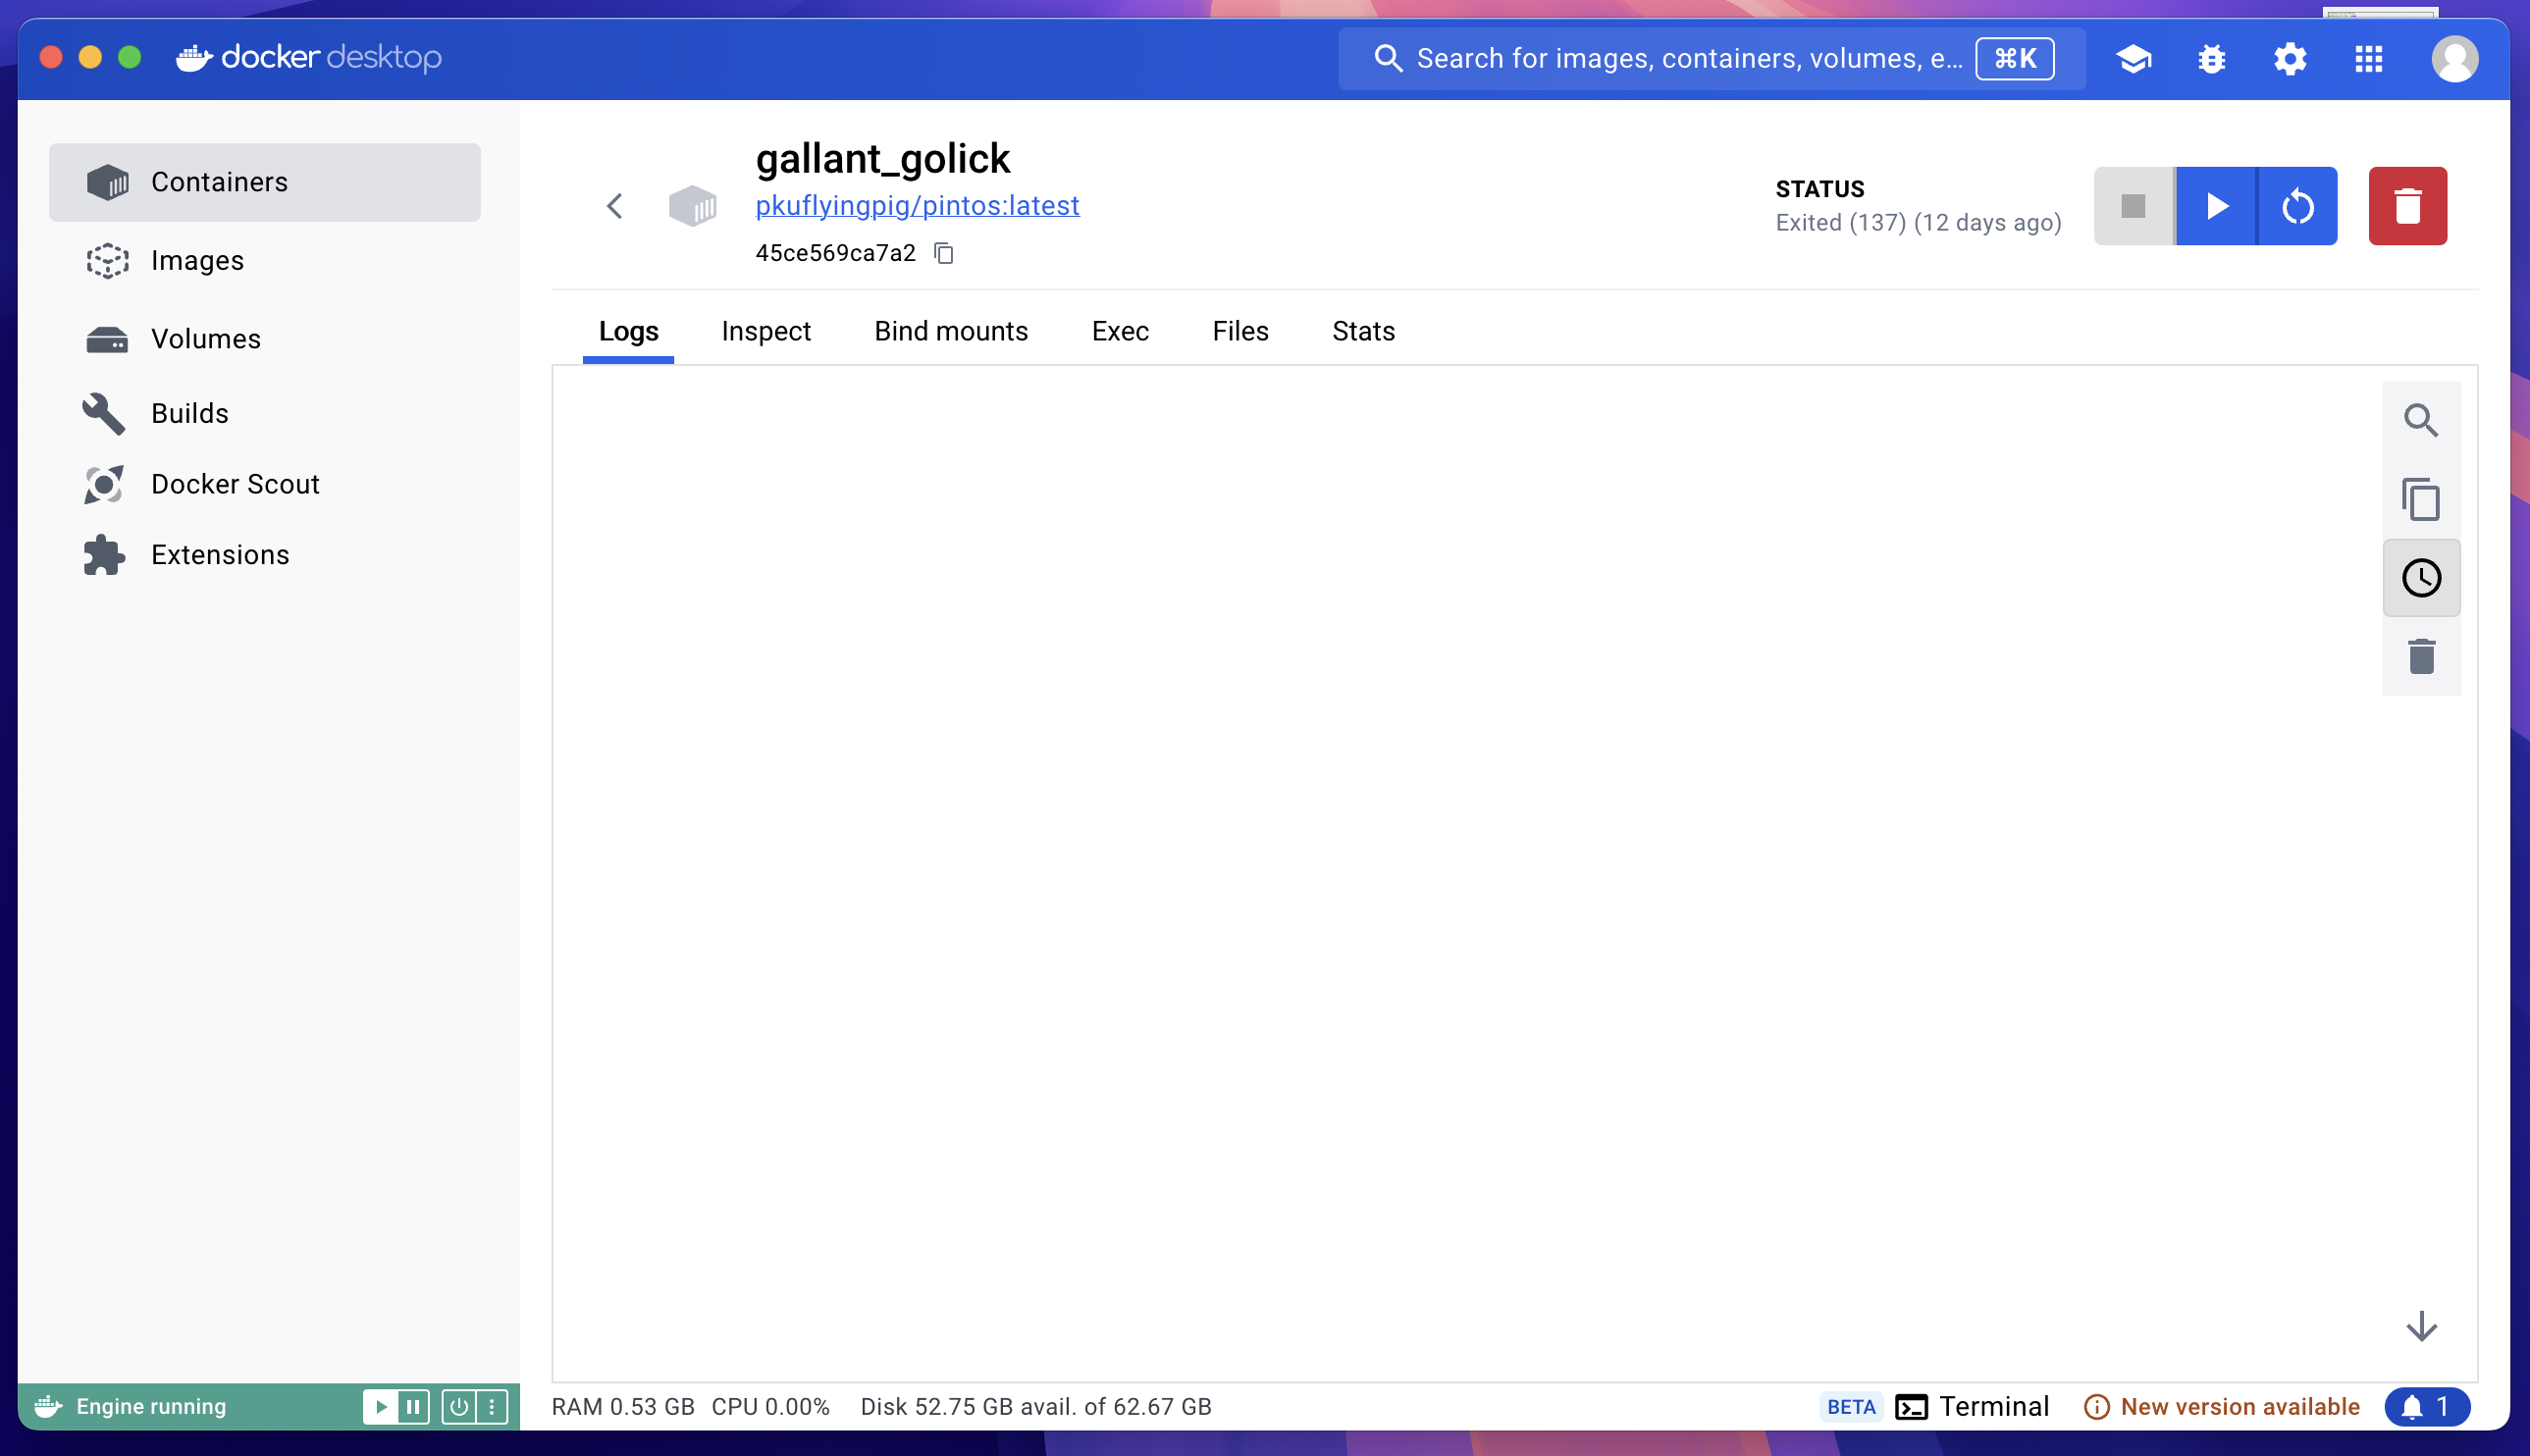
\includegraphics[width=0.9\textwidth]{img/docker_install.png}
	\caption{Docker容器}
\end{figure}

\subsection{专用服务器}

专用服务器的系统环境如下表所示:

\begin{center}
	\begin{tabular}{| >{\centering\arraybackslash}m{3cm} | >{\centering\arraybackslash}m{9cm} |}    
		\hline  
		\textbf{项目名称} & \textbf{详细信息} \\
		\hline  
		操作系统 & Ubuntu 22.04 LTS \\  
		\hline  
		系统类型 & 64位操作系统,基于x64的处理器 \\  
		\hline
		CPU & 14th Gen Intel(R) Core(TM) i9-14900K 3.20 GHz \\  
		\hline 
		GPU & NVIDIA GeForce RTX 4090 D (24GB)\\  
		\hline 
		内存 & 64GB DDR5 4800MHz \\  
		\hline 
		磁盘 & 4TB SSD \\  
		\hline 		
	\end{tabular}
\end{center}

通过\texttt{ssh}远程连接后,服务器正常运行,如下图所示:

\begin{figure}[H]
	\centering
	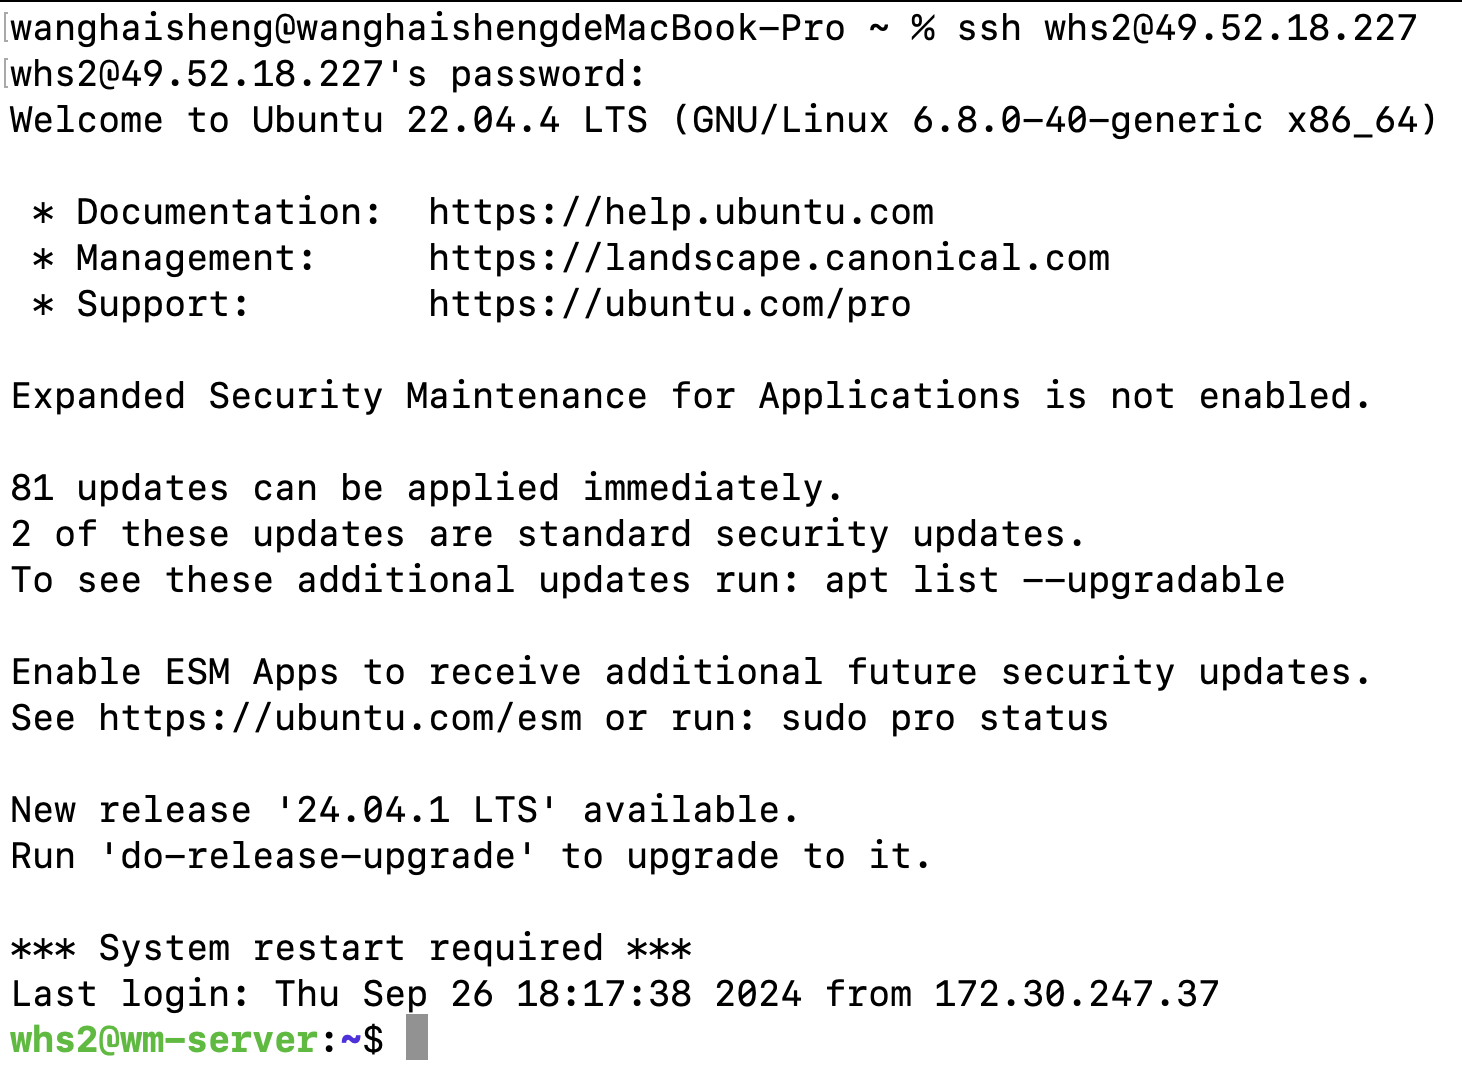
\includegraphics[width=0.9\textwidth]{img/server_init.png}
	\caption{专用服务器}
\end{figure}

\subsection{Windows Subsystem for Linux (WSL)}

WSL系统环境如下表所示:

\begin{center}
	\begin{tabular}{| >{\centering\arraybackslash}m{3cm} | >{\centering\arraybackslash}m{9cm} |}    
		\hline  
		\textbf{项目名称} & \textbf{详细信息} \\
		\hline  
		操作系统 & Windows 11 专业版 23H2 \\  
		\hline  
		系统类型 & 64位操作系统,基于x64的处理器 \\  
		\hline
		CPU & 12th Gen Intel(R) Core(TM) i7-12800HX 2.00 GHz \\  
		\hline 
		GPU & NVIDIA GeForce RTX 3080 Ti Laptop (16GB)\\  
		\hline 
		内存 & 32GB DDR5 4800MHz \\  
		\hline 
		磁盘 & 1TB SSD \\  
		\hline 		
	\end{tabular}
\end{center}

使用\texttt{wsl --list --online}命令查看可用版本,再使用\texttt{wsl.exe --install Ubuntu-18.04}命令安装Ubuntu 18.04。稍等片刻后,WSL正常运行,如下图所示:

\begin{figure}[H]
	\centering
	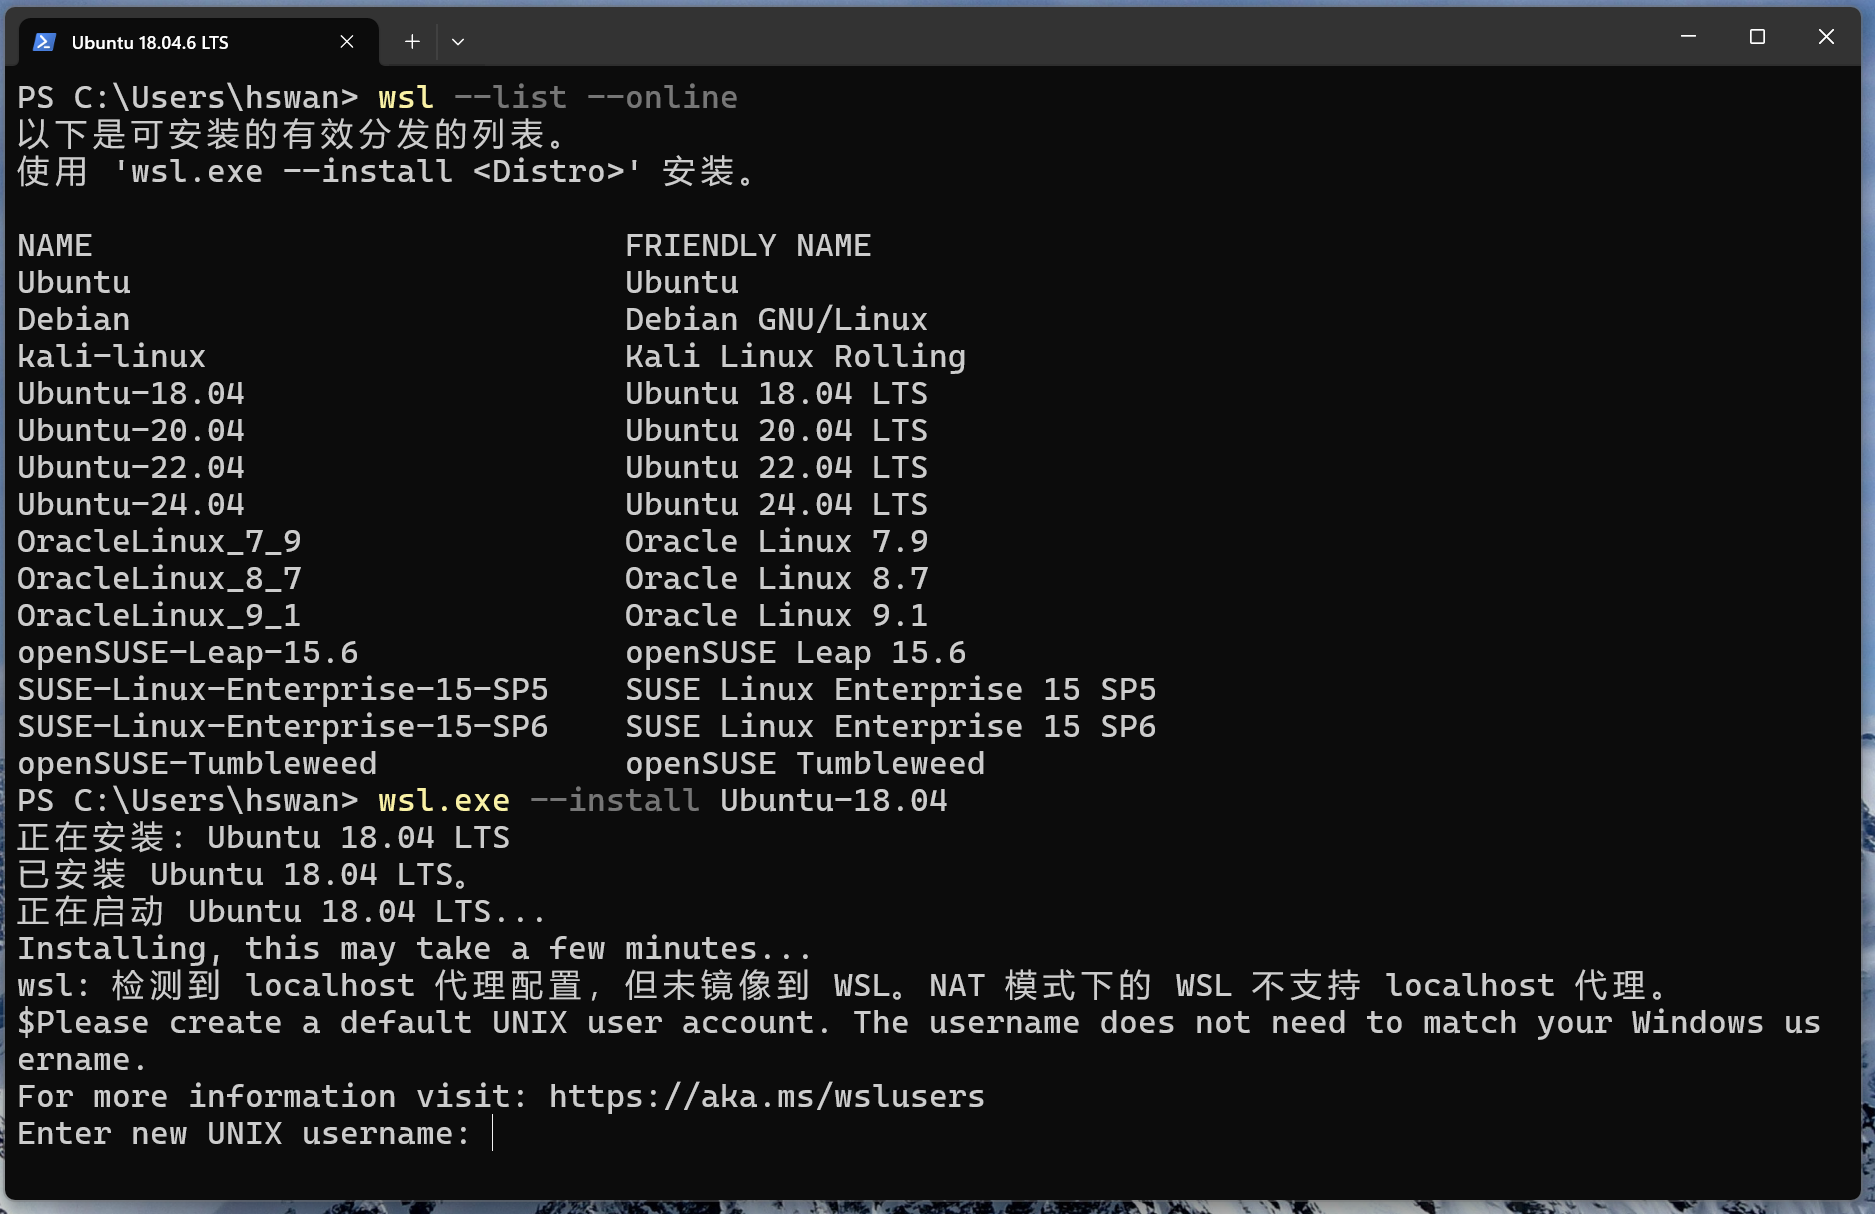
\includegraphics[width=0.9\textwidth]{img/wsl_install.png}
	\caption{WSL}
\end{figure}

\normalsize

\section{实验过程}

在本次实验中,我依次尝试了四种方法安装运行PintOS,除专用服务器外的四种方法都成功了。具体过程如下所示。

\subsection{Virtualbox虚拟机}

首先,下载大夏学堂上的虚拟电脑软件包 \texttt{OS.ova}, 导入Virtualbox虚拟机,如下图所示。所有配置均为默认配置,包括双核处理器,4GB虚拟内存,20GB虚拟磁盘等。

\begin{figure}[H]
	\centering
	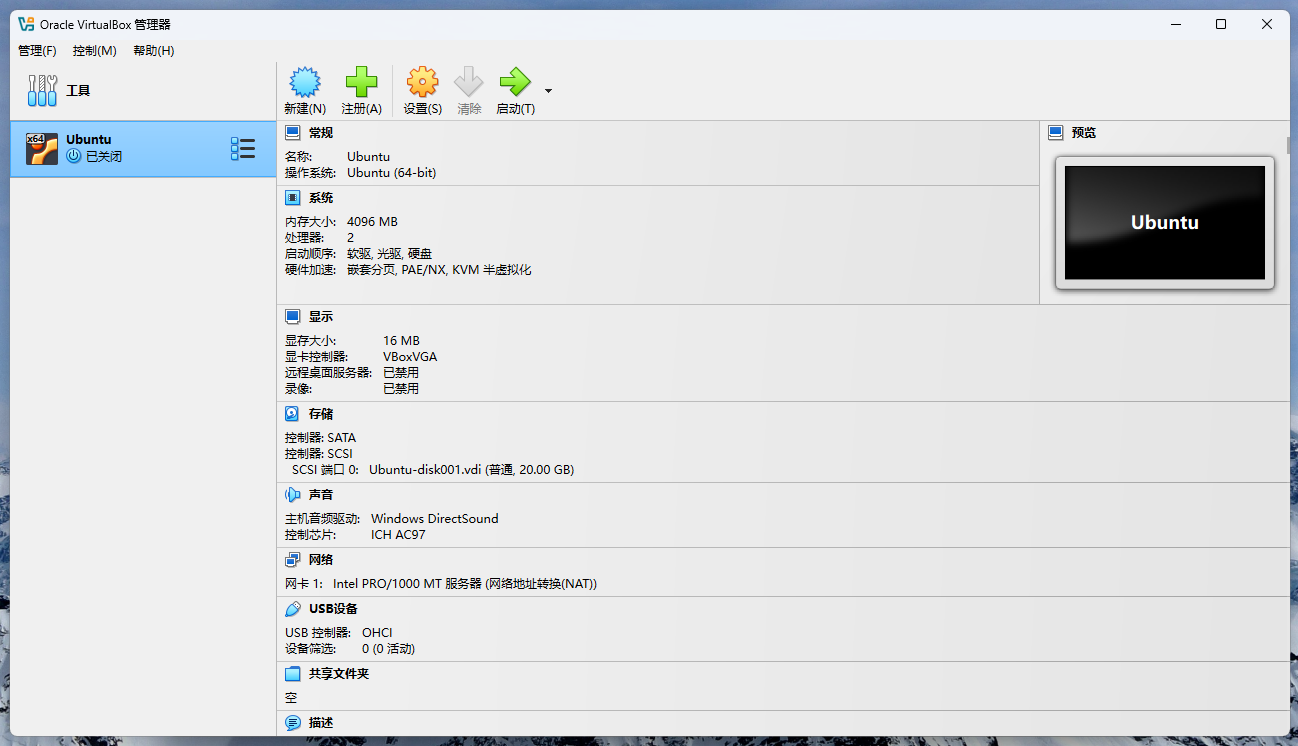
\includegraphics[width=0.9\textwidth]{img/virtualbox_computer_loaded.png}
	\caption{在Virtualbox虚拟机中导入虚拟电脑}
\end{figure}

启动后,虚拟机正常运行,但显示分辨率仅为 \texttt{720*540},无法有效显示信息。使用键盘快捷键\texttt{Ctrl + Alt + T}打开命令行,使用 \texttt{xrandr} 命令设置分辨率为 \texttt{2560*1440},充满整个屏幕,如下图。

\begin{figure}[H]
	\centering
	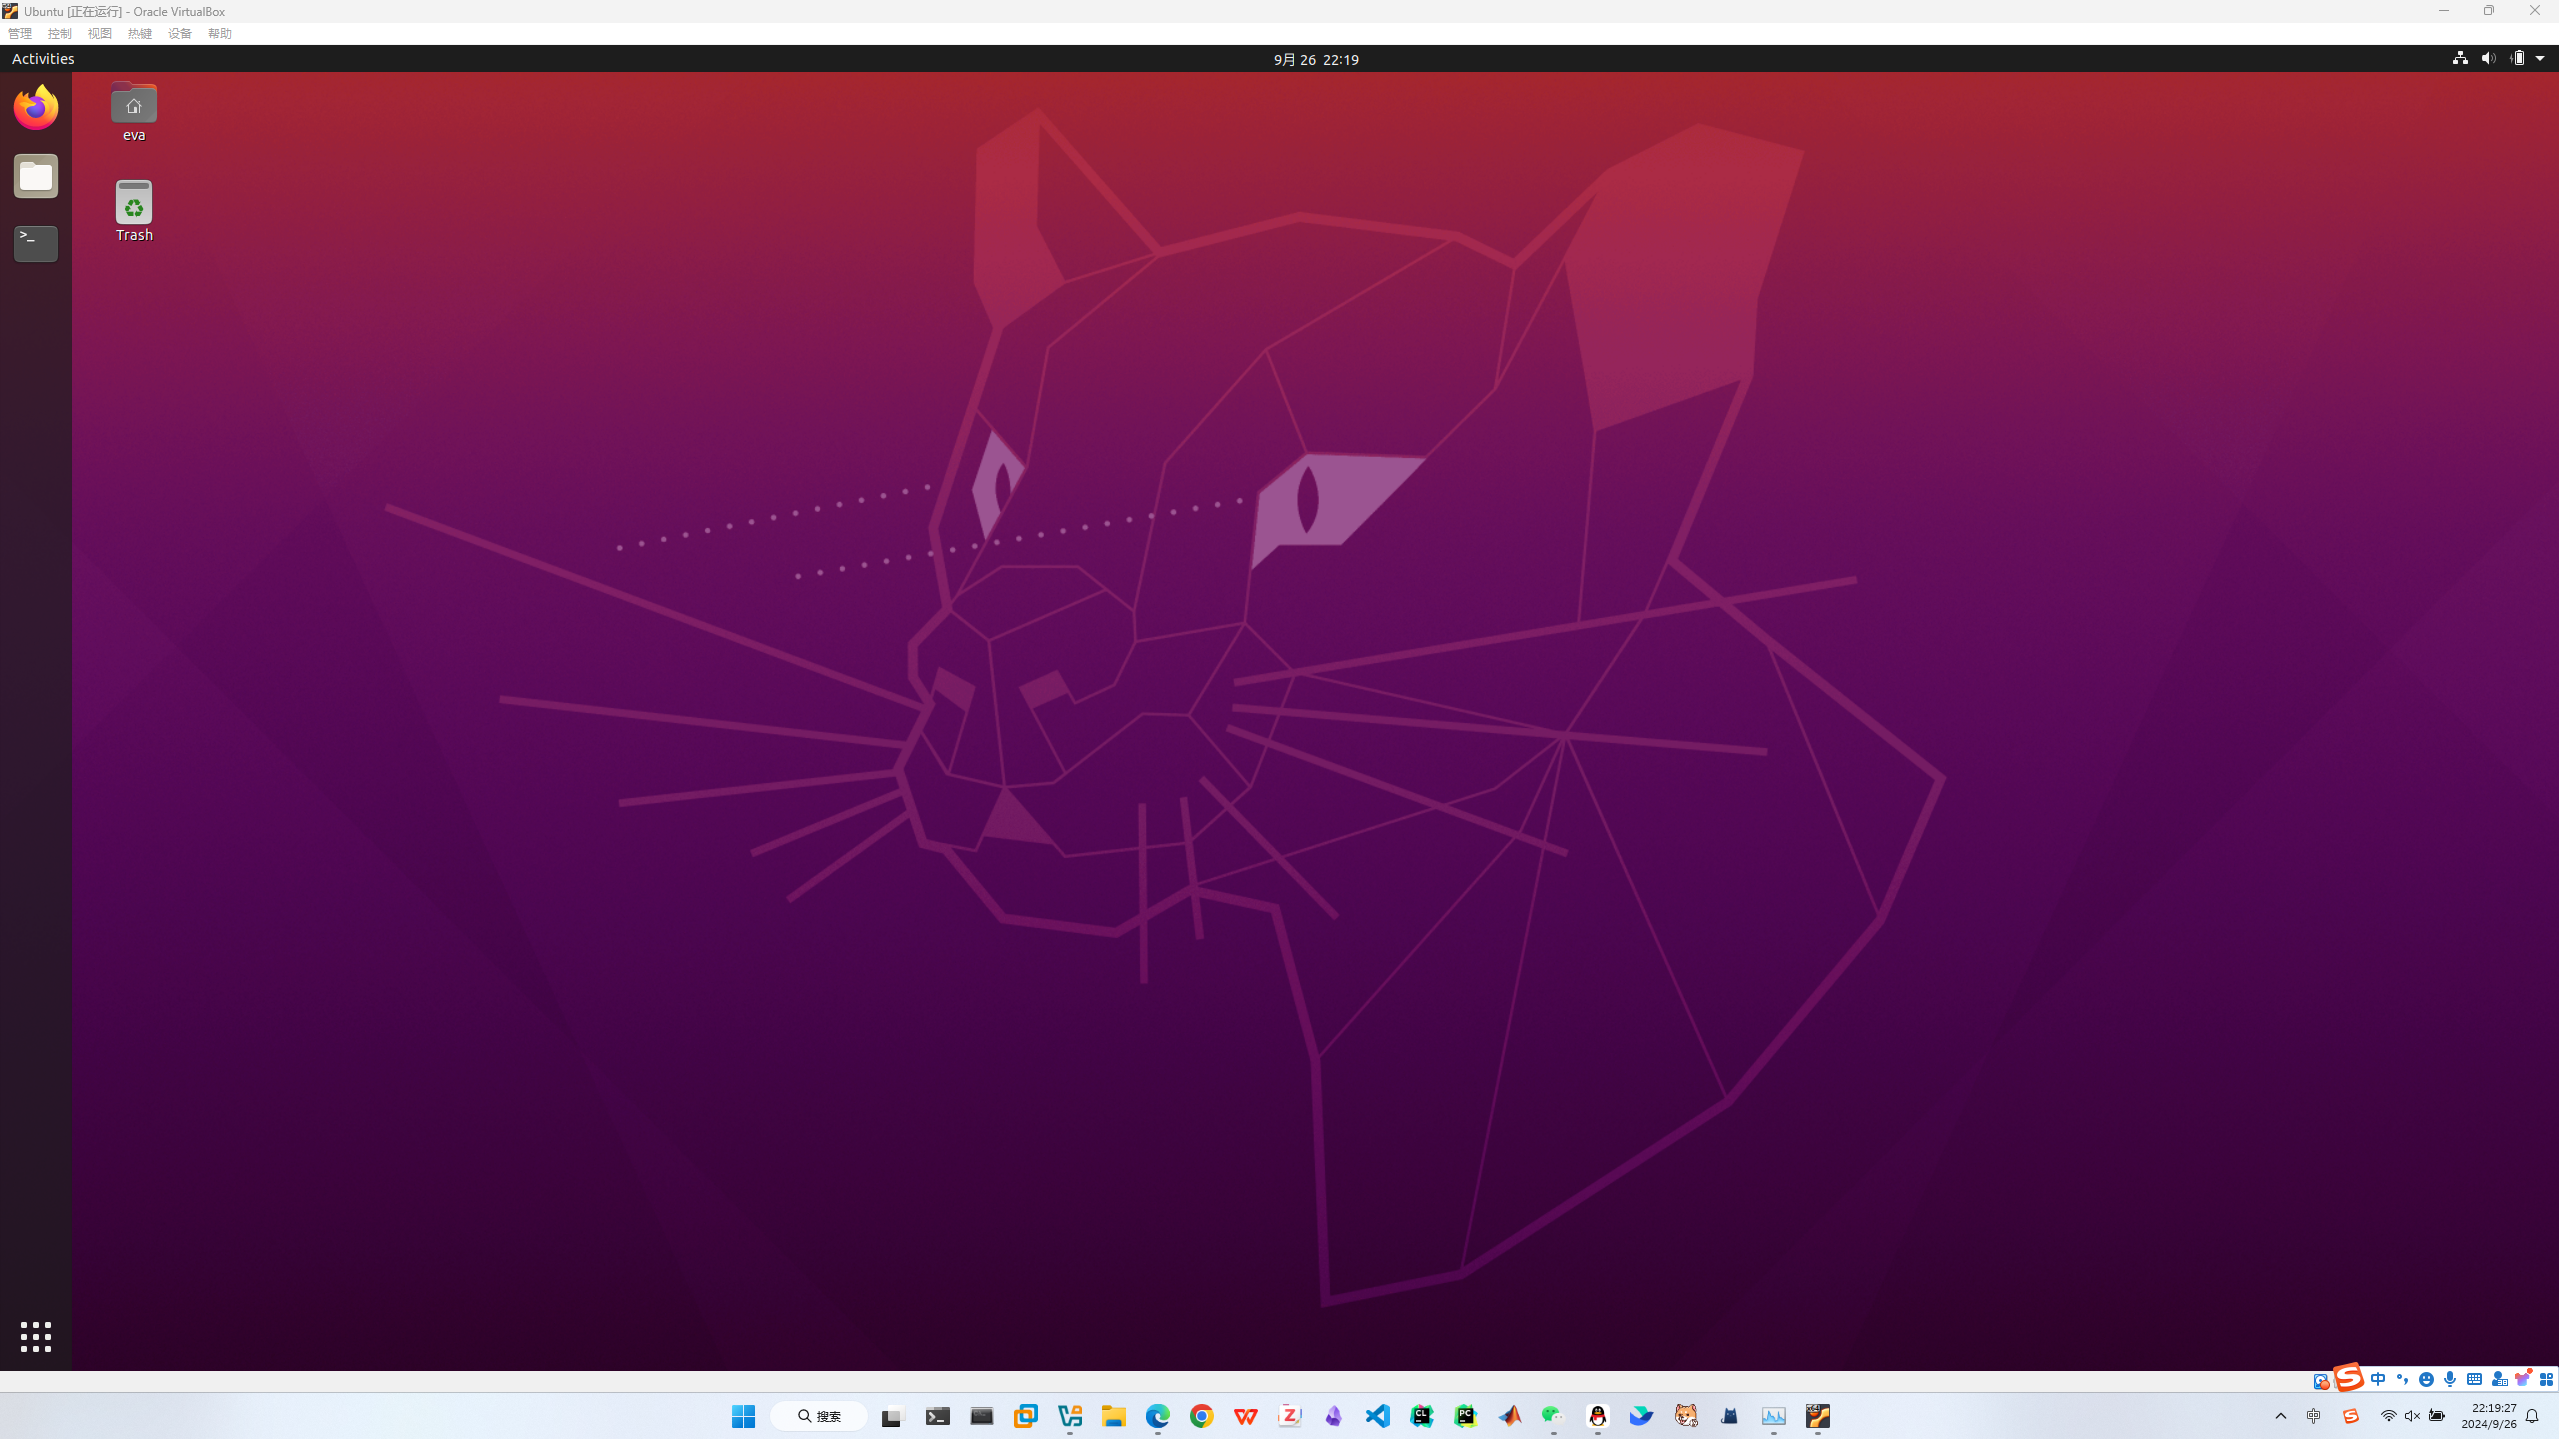
\includegraphics[width=0.9\textwidth]{img/ubuntu_desktop_virtualbox.png}
	\caption{运行虚拟电脑并调整至正常分辨率}
\end{figure}

接着打开命令行,按照教程进入 \texttt{~/pintos/src/threads} 文件目录,并执行 \texttt{make} 命令。然而,这个文件已经编译完成,故提示 \texttt{Nothing to be done for 'all'.}。运行情况如图所示。

\begin{figure}[H]
	\centering
	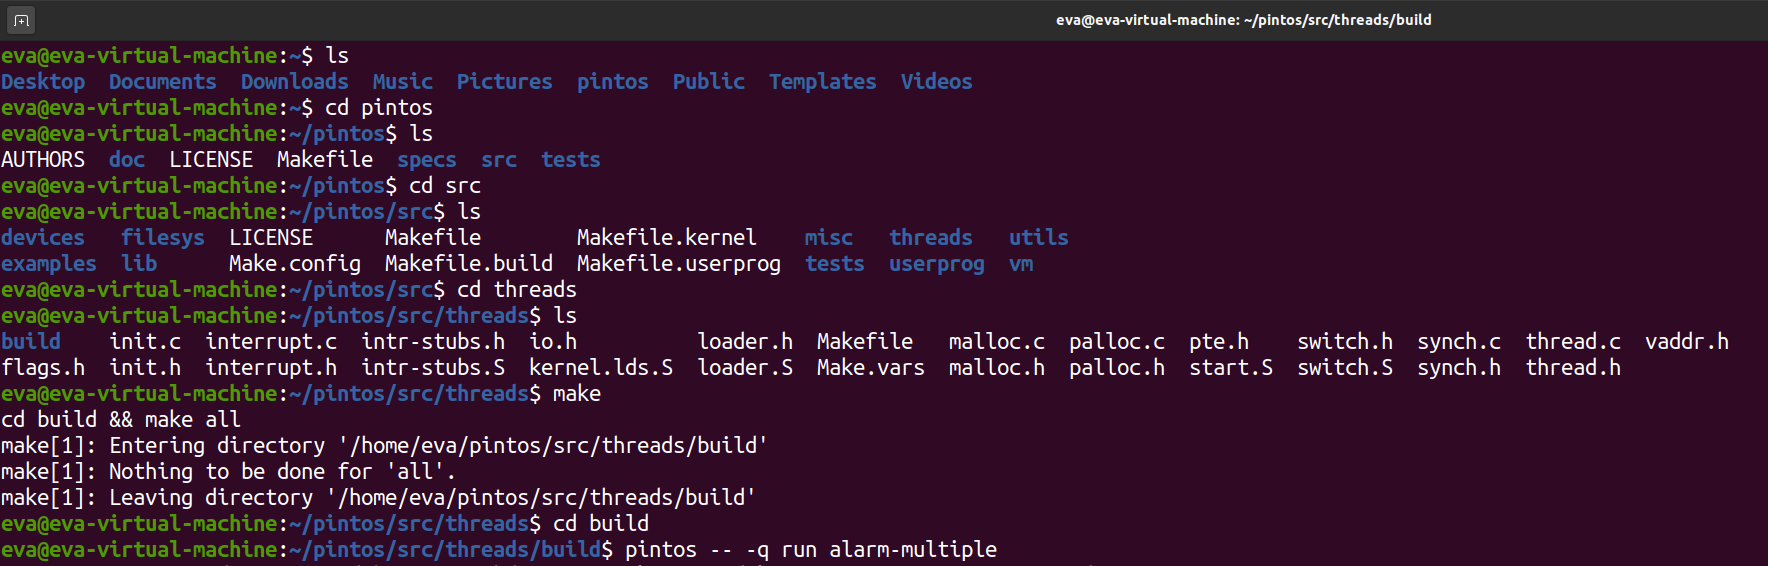
\includegraphics[width=0.9\textwidth]{img/make_virtualbox.png}
	\caption{编译运行PintOS}
\end{figure}

最后进入 \texttt{build} 文件目录,并执行 \texttt{pintos -- -q run alarm-multiple} 命令。运行结果如下:

\begin{figure}[H]
	\centering
	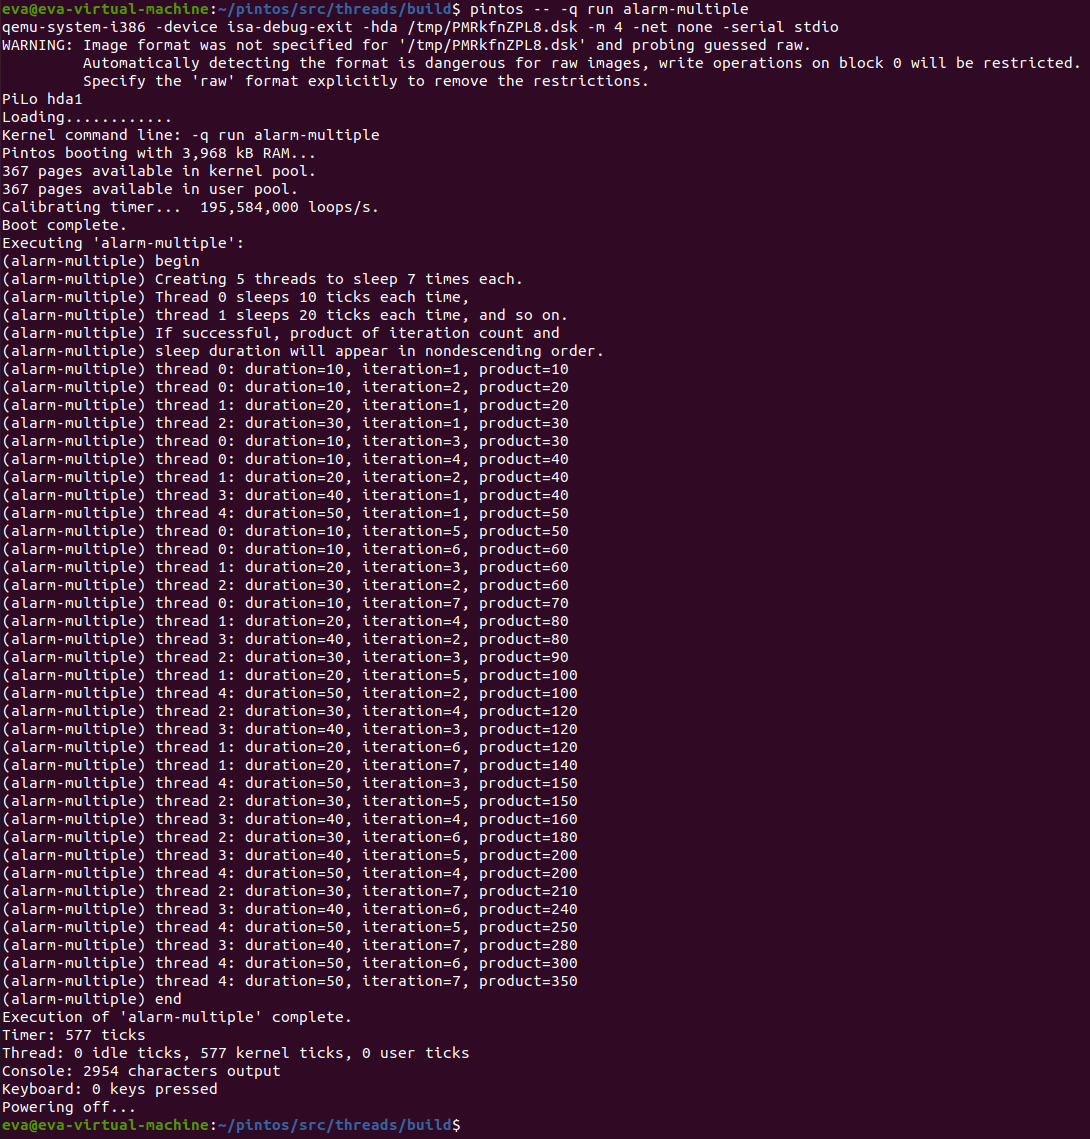
\includegraphics[width=0.9\textwidth]{img/result_virtualbox.png}
	\caption{最终运行结果}
\end{figure}

至此,Virtualbox虚拟机已经成功安装并运行PintOS。

\subsection{Docker容器}

首先,使用\texttt{docker run -it pkuflyingpig/pintos bash}命令拉取Docker镜像。

接下来的步骤和前面的方法相似:先从GitHub拉取镜像,再进入\texttt{pintos/src/threads}文件夹,执行\texttt{make}编译指令,最后输入\texttt{pintos -- -q run alarm-multiple}命令查看结果。如下图所示。

\begin{figure}[H]
	\centering
	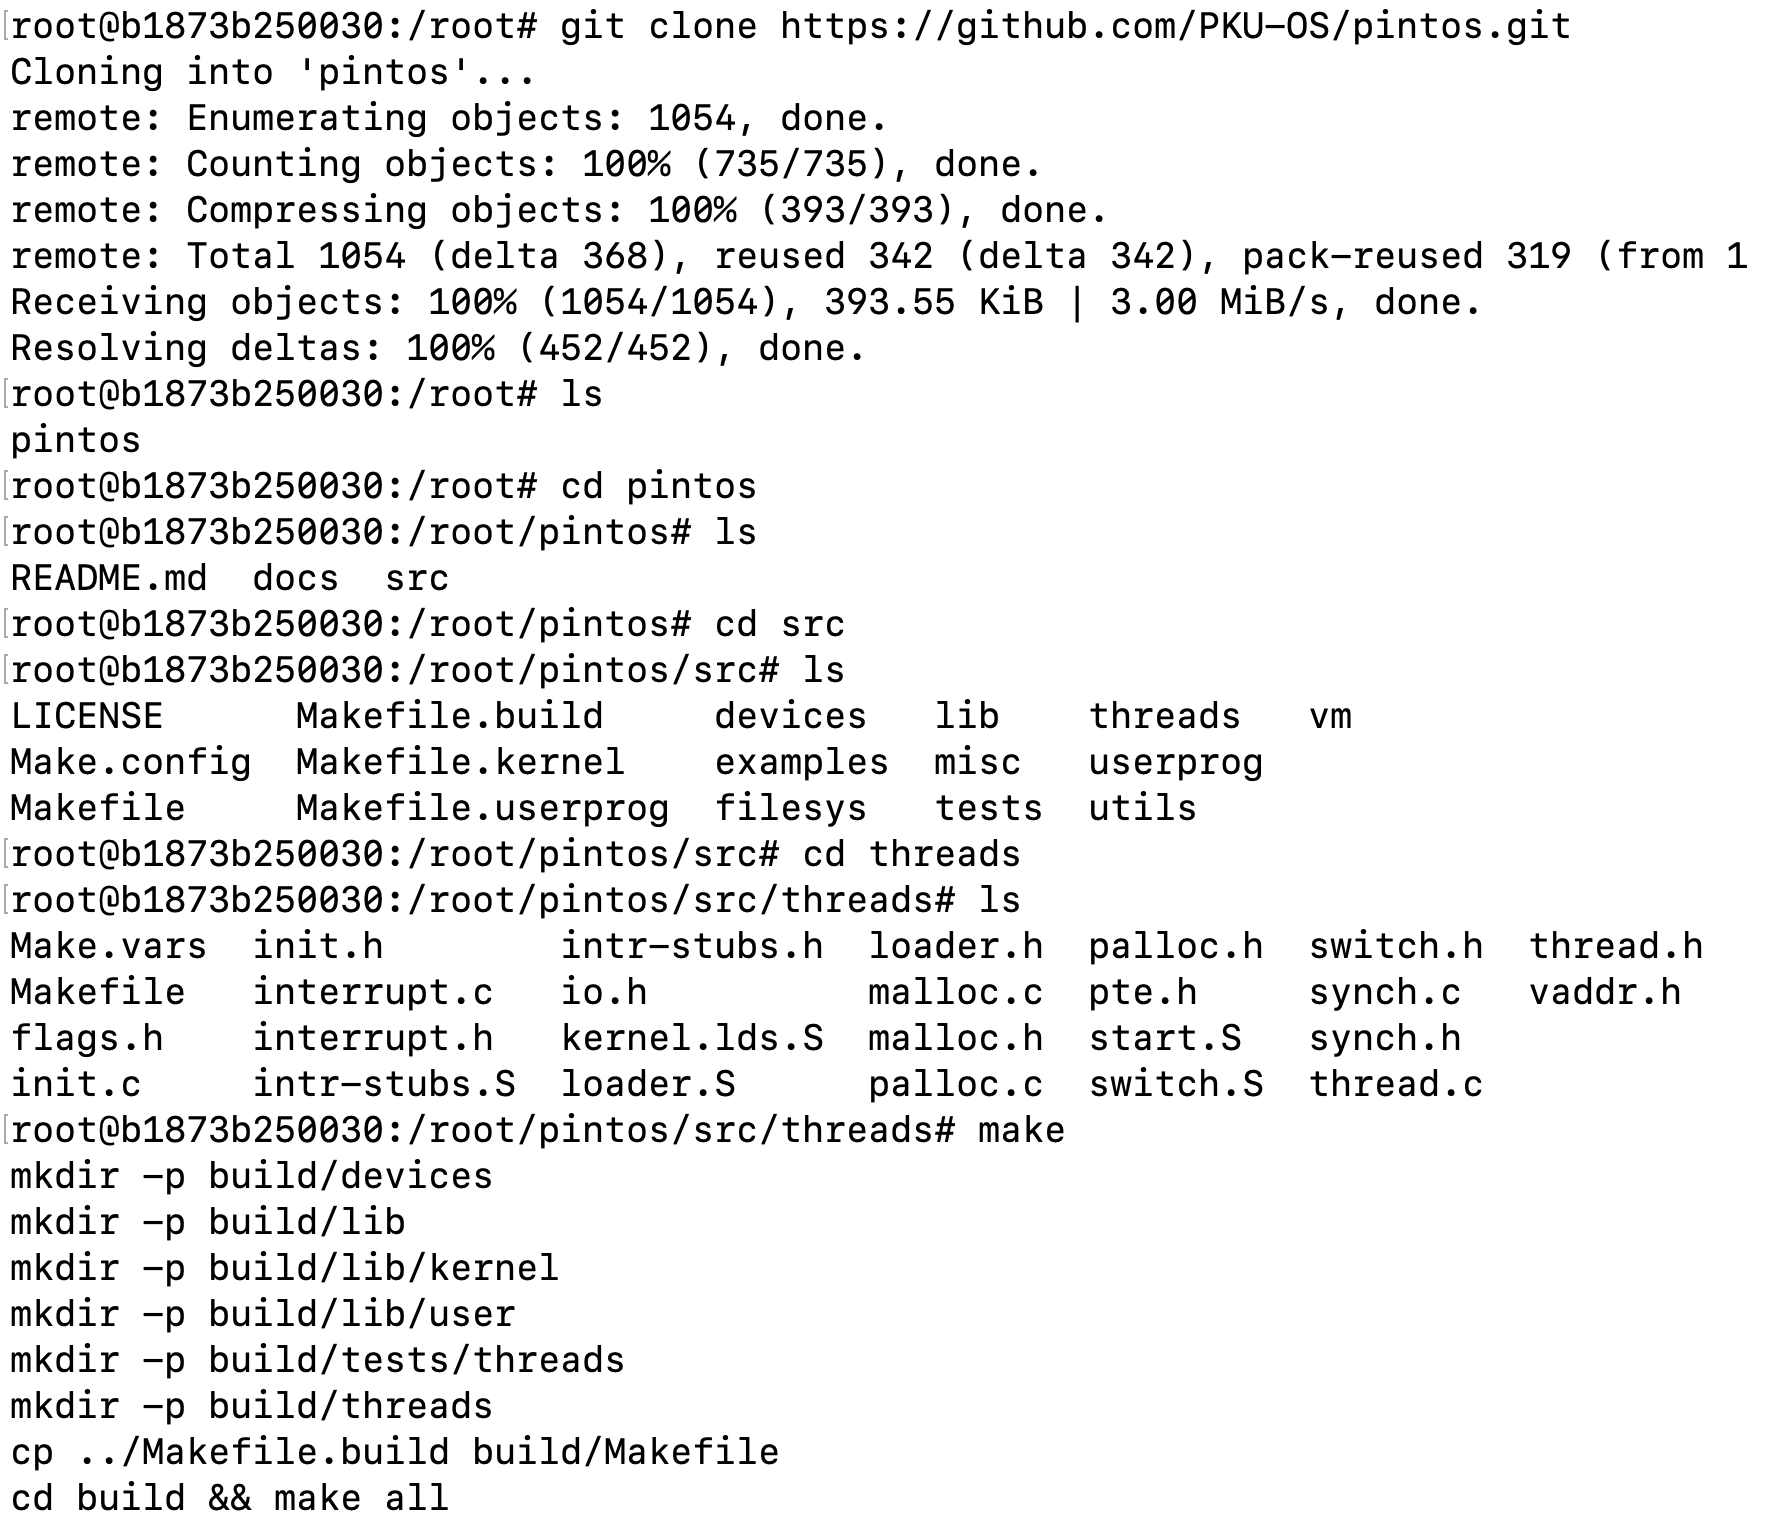
\includegraphics[width=0.9\textwidth]{img/docker_make_try.png}
	\caption{Docker直接编译PintOS}
\end{figure}

然而,这里出现了\texttt{rosetta error},即转译错误,如下图所示。

\begin{figure}[H]
	\centering
	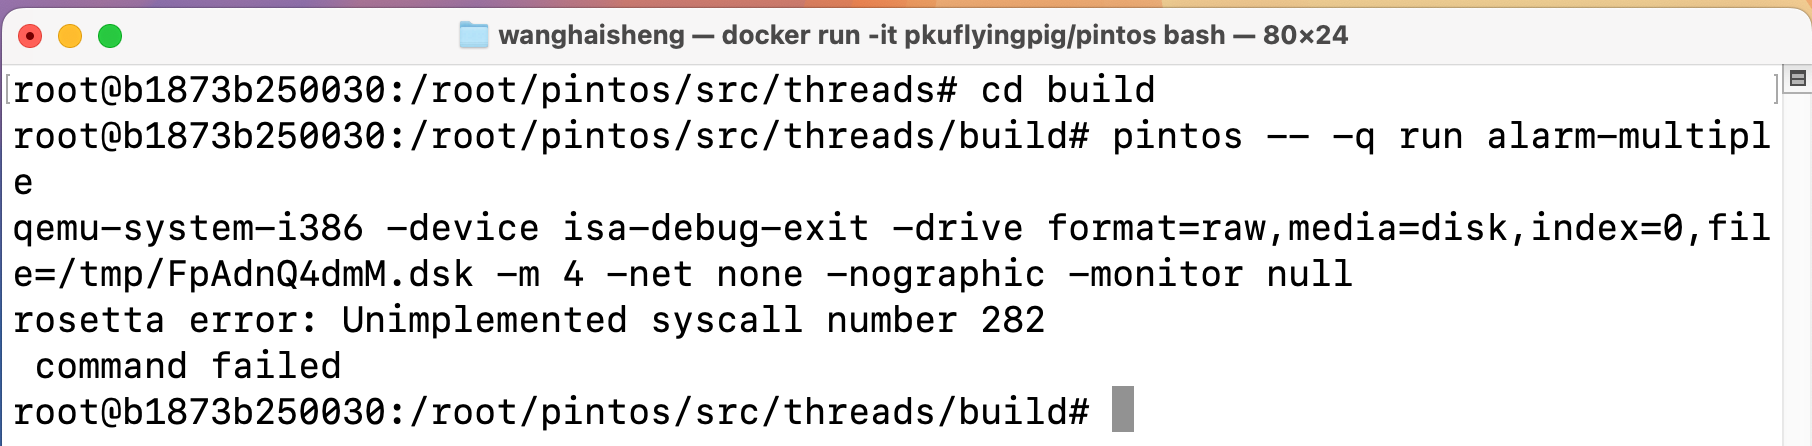
\includegraphics[width=0.9\textwidth]{img/docker_make_fail.png}
	\caption{Docker出现转译错误}
\end{figure}

Rosetta是苹果电脑上的一种翻译器,使基于x86架构的应用程序能够在Apple Silicon(如M1芯片)上运行,实现跨处理器架构的应用程序兼容性。Rosetta并不完美,在涉及底层架构的指令上有时会出现兼容性问题,比如当前遇到的情况。为了克服这一缺陷,我们关闭Rosetta转译系统,如下图。

\begin{figure}[H]
	\centering
	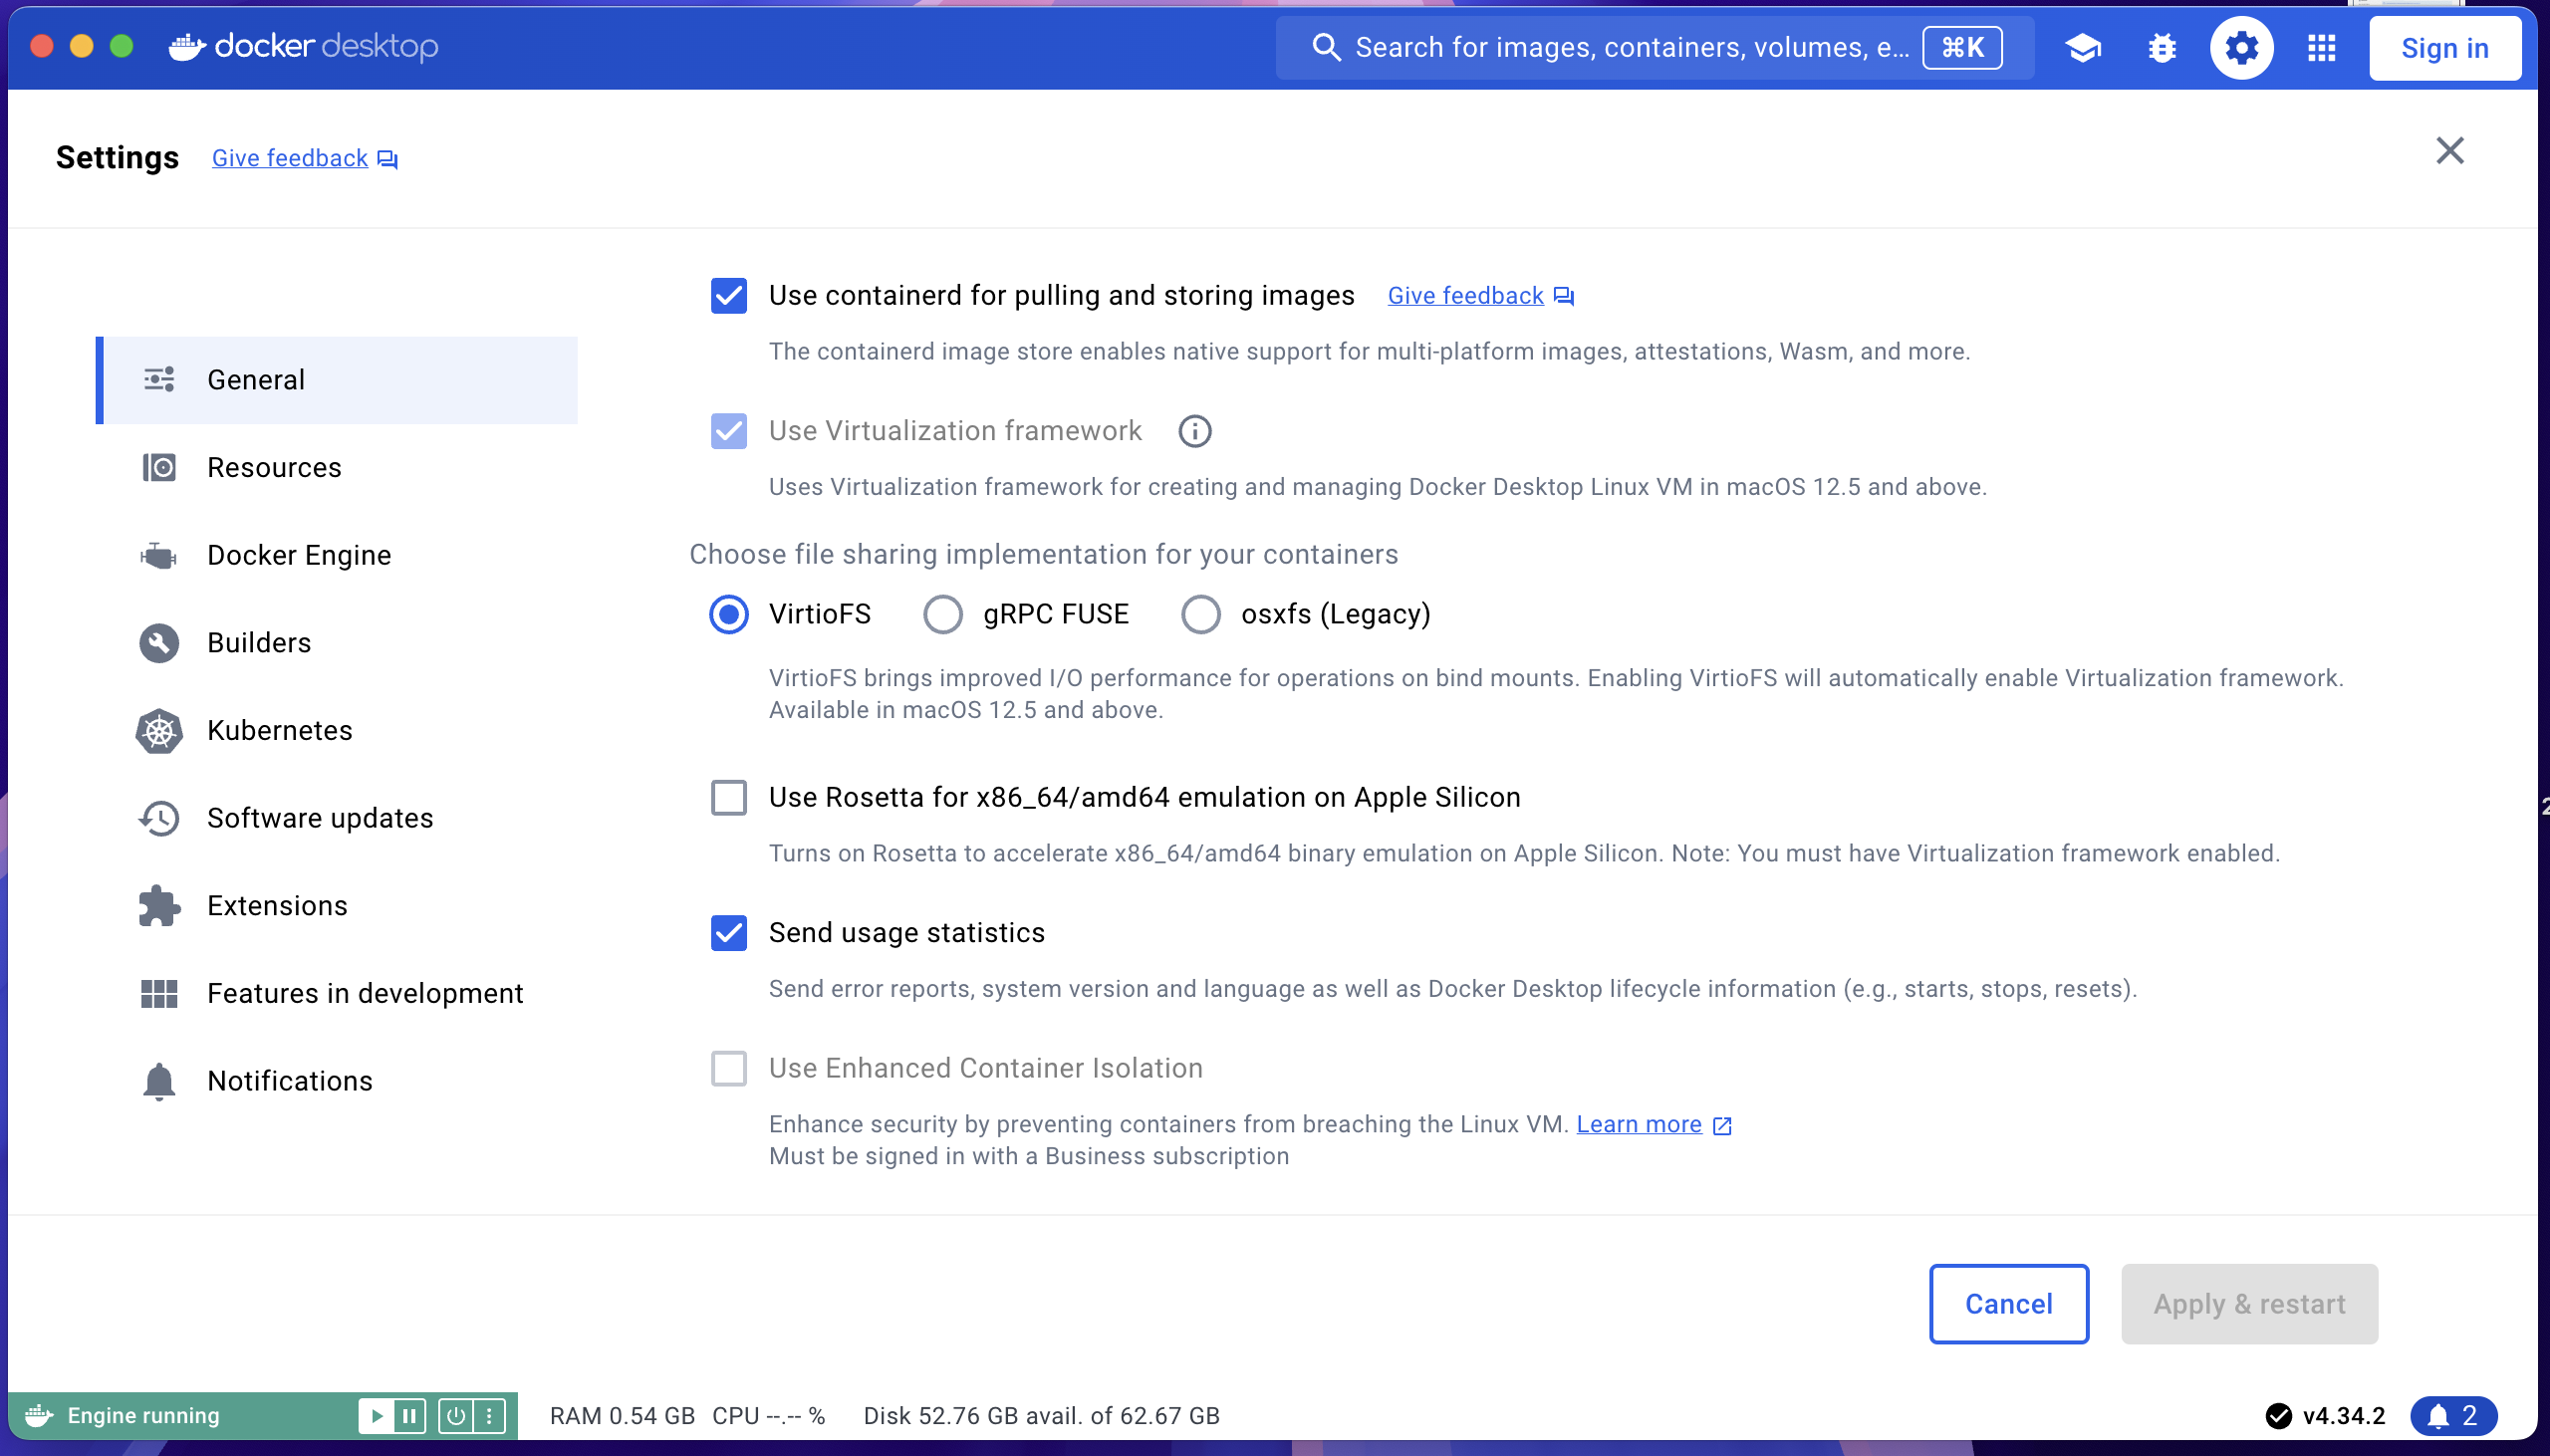
\includegraphics[width=0.9\textwidth]{img/docker_setup.png}
	\caption{关闭Docker的Rosetta优化}
\end{figure}

在这种情况下,Docker直接以兼容模式运行(x86架构程序运行在ARM芯片上)。我们重新编译PintOS的源码,如下图所示。

\begin{figure}[H]
	\centering
	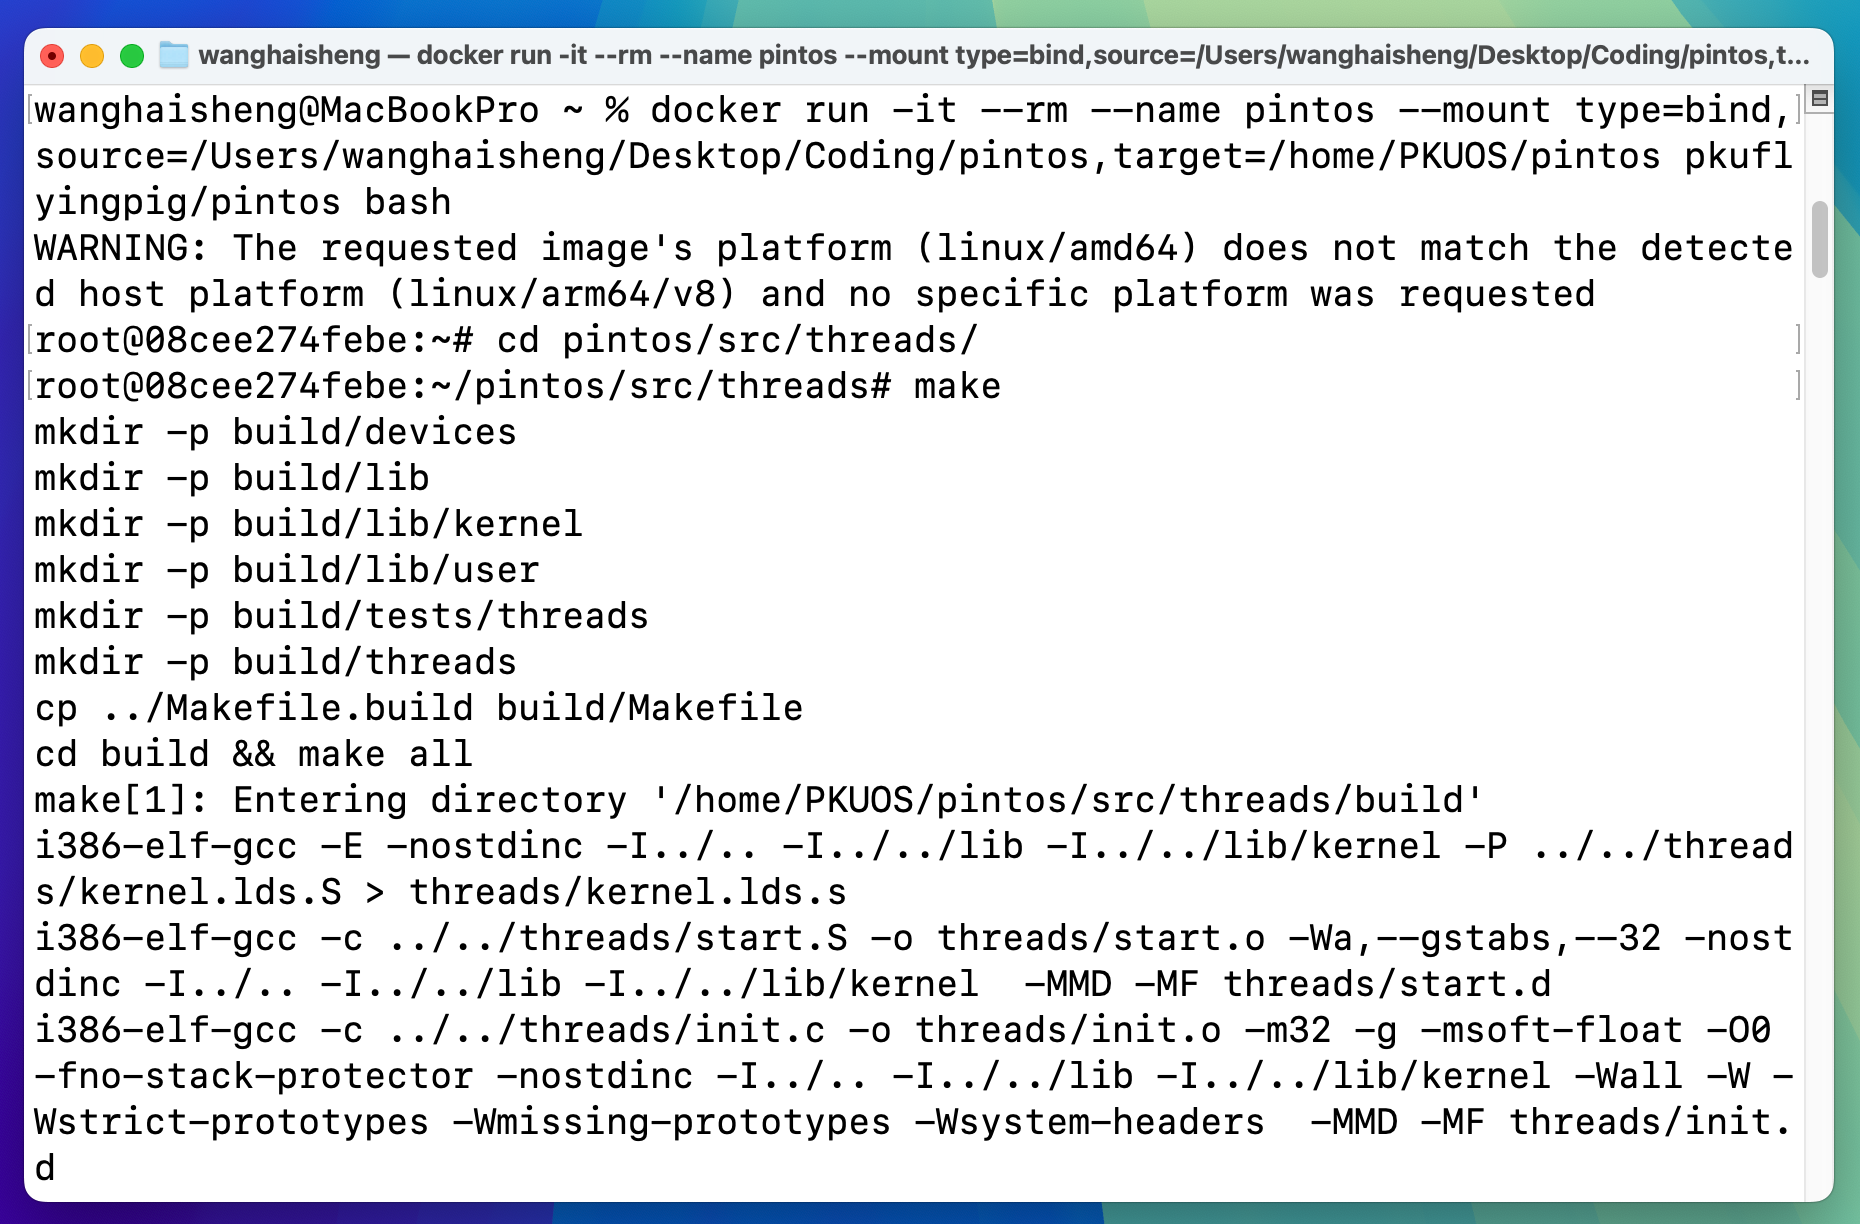
\includegraphics[width=0.9\textwidth]{img/docker_make.png}
	\caption{重新编译PintOS源码}
\end{figure}

接着运行\texttt{pintos -- -q run alarm-multiple}命令,结果如下:

\begin{figure}[H]
	\centering
	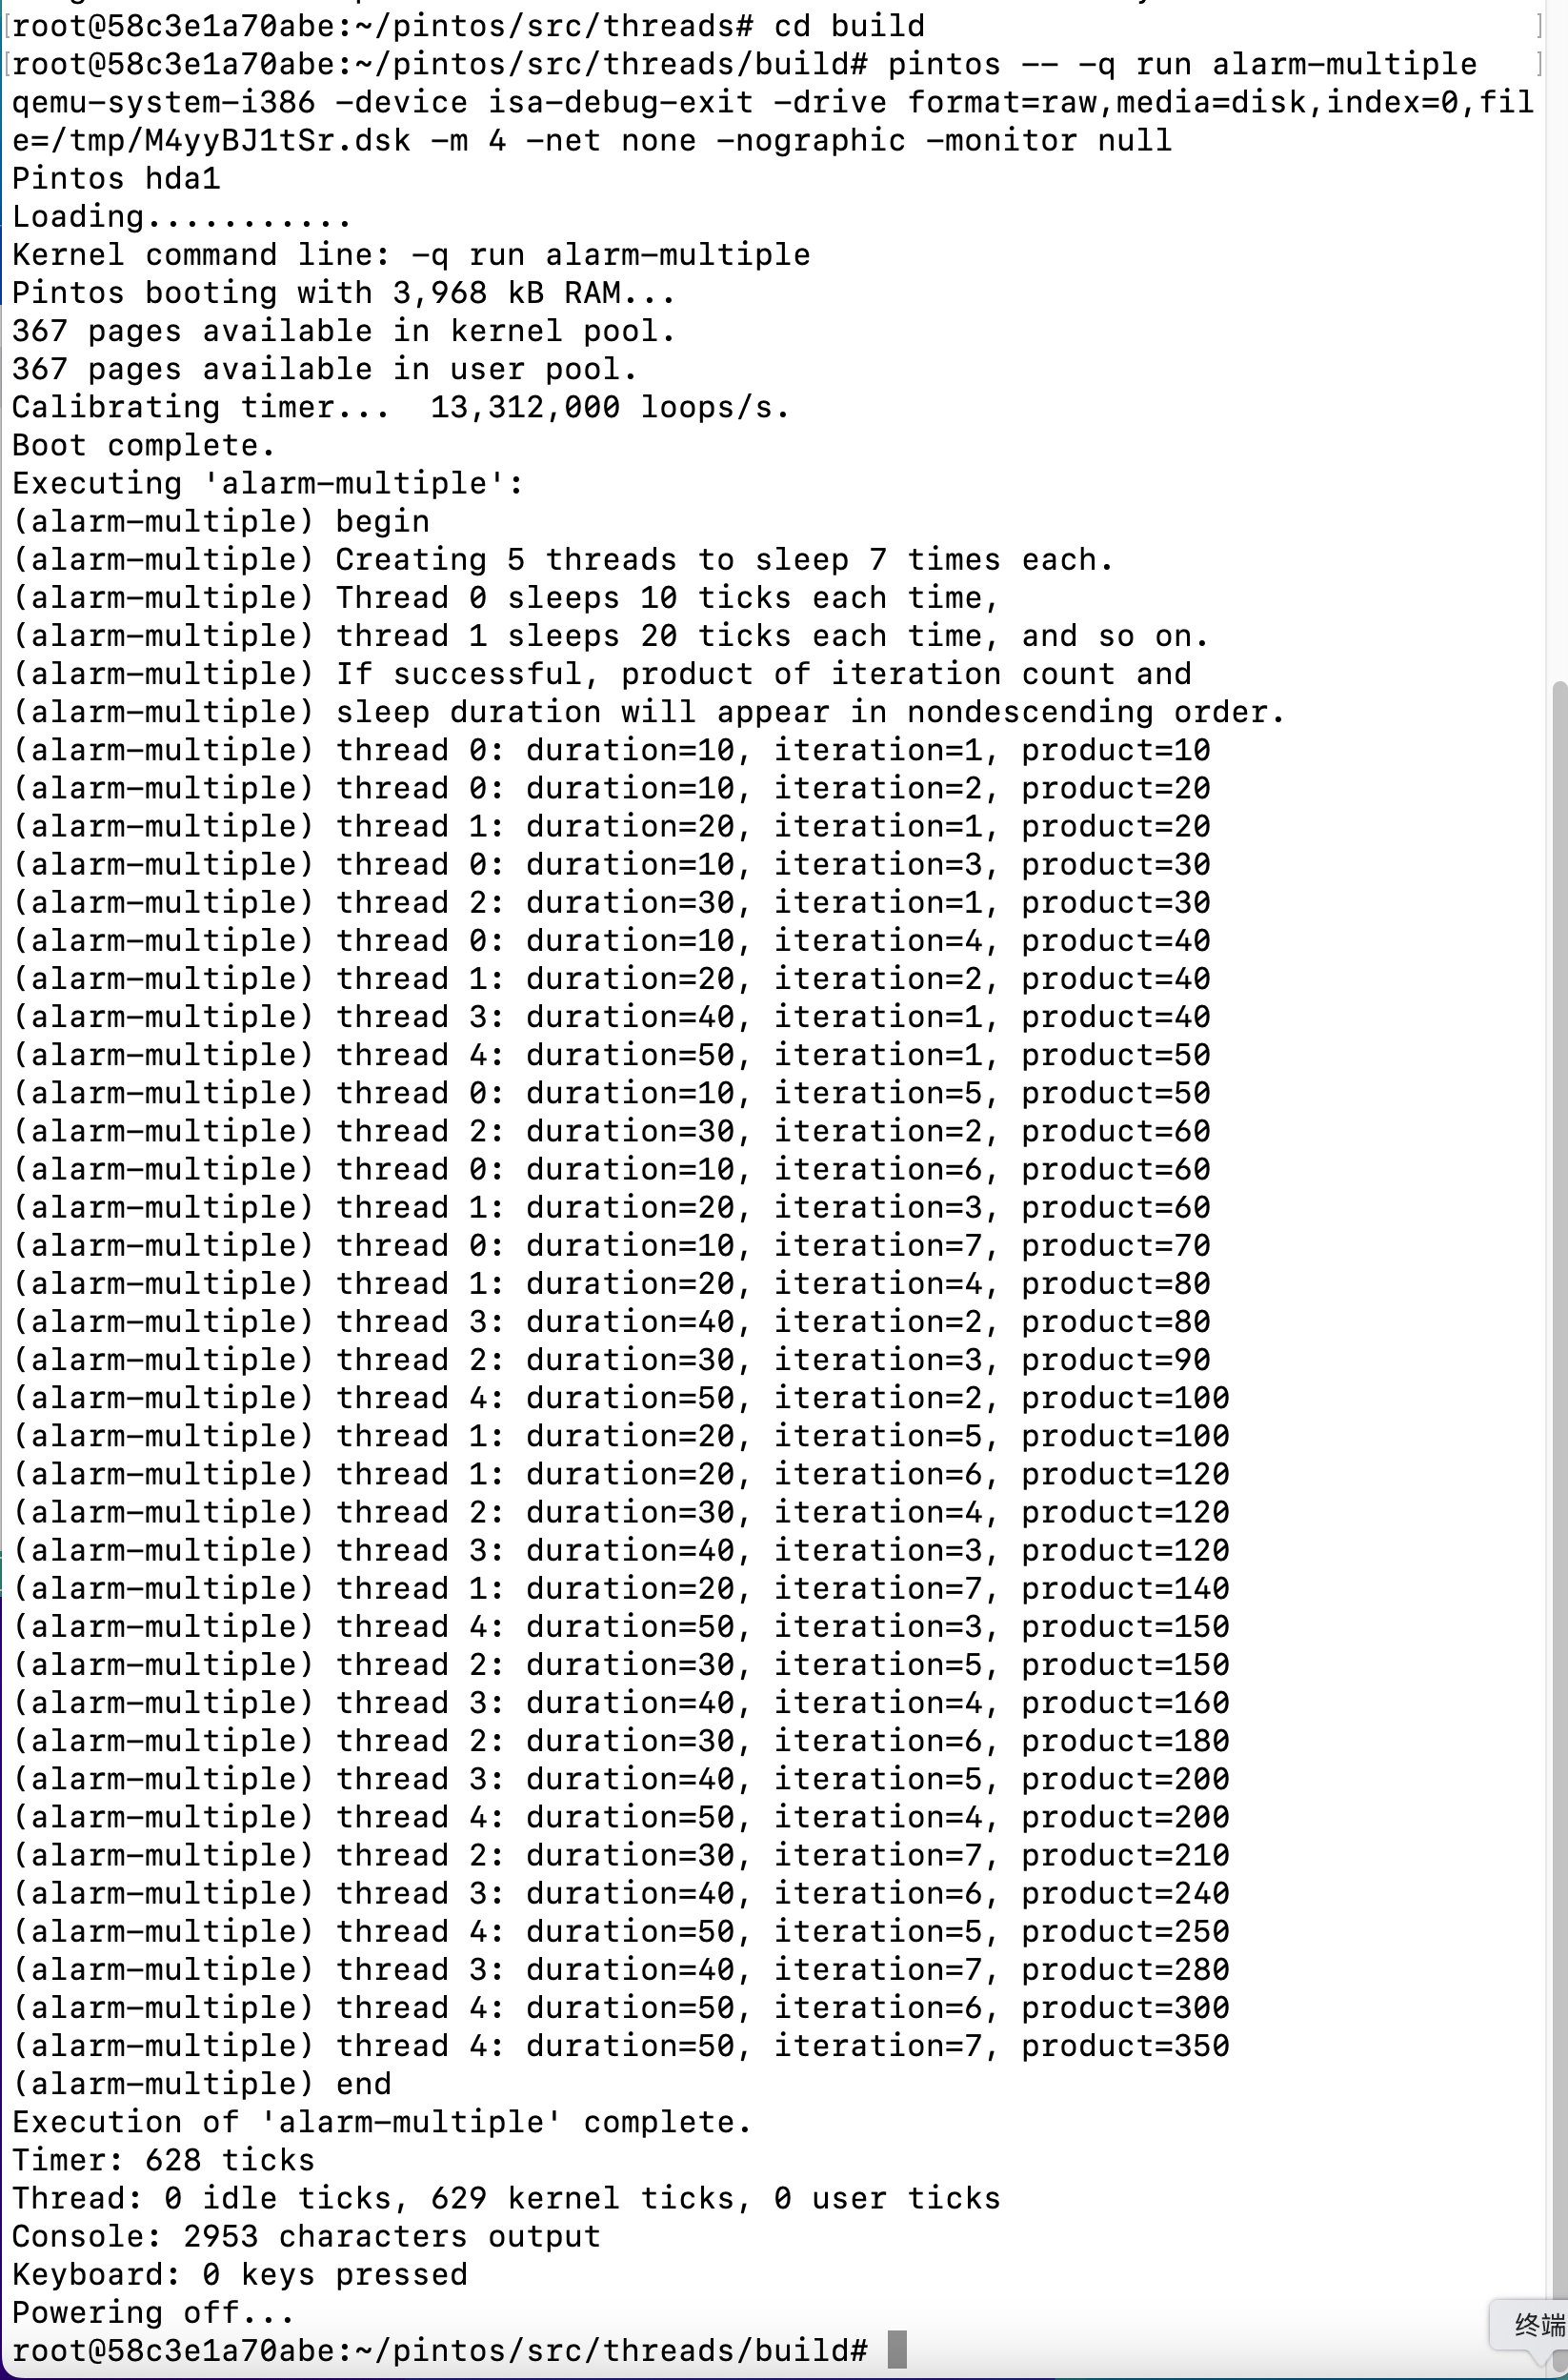
\includegraphics[width=0.9\textwidth]{img/docker_result.png}
	\caption{最终运行结果}
\end{figure}

由于Docker的设计初衷是快速部署,所以Docker在文件管理方面比较麻烦。如果使用后直接关闭容器,所做更改不会被保存,一不小心就前功尽弃。有一种办法是将更改作为一个新的镜像保存,但这样很浪费磁盘空间。最后,我选择了文件挂载的方法——将\texttt{pintos}文件夹放在我的宿主操作系统中,然后挂载到Docker容器中。这样,每次的更改都会被保存在宿主系统中,既方便保存,又节约了磁盘空间。

使用的命令如下:\texttt{docker run -it --rm --name pintos --mount type=bind,source=/Users/wanghaisheng/Desktop/Coding/pintos,target=/home/PKUOS/pintos pkuflyingpig/pintos bash}

这条命令的具体含义如下表:

\begin{center}
	\begin{tabular}{| >{\centering\arraybackslash}m{6cm} | >{\centering\arraybackslash}m{9cm} |}  
		\hline  
		\textbf{命令} & \textbf{含义} \\  
		\hline  
		docker run & 运行一个新的Docker容器 \\  
		\hline  
		-it & 以交互模式运行容器,允许通过终端与容器交互 \\  
		\hline  
		-i & 使容器保持标准输入开放 \\  
		\hline  
		-t & 为容器分配一个伪终端 \\  
		\hline  
		--rm & 当容器停止时自动删除容器,避免占用系统资源 \\  
		\hline  
		--name pintos & 给容器命名为\texttt{pintos},方便管理 \\  
		\hline  
		--mount type=bind,source=... & 将主机上的一个目录绑定挂载到容器内的指定目录 \\  
		\hline  
		type=bind & 指定挂载类型为绑定挂载 \\  
		\hline  
		source=... & 主机上挂载文件的实际路径 \\  
		\hline  
		target=/home/PKUOS/pintos & 容器内的挂载路径 \\  
		\hline  
		pkuflyingpig/pintos & 指定要使用的Docker镜像 \\  
		\hline  
		bash & 在容器内执行\texttt{bash}命令,进入Bash shell \\  
		\hline  
	\end{tabular}
\end{center}

\begin{figure}[H]
	\centering
	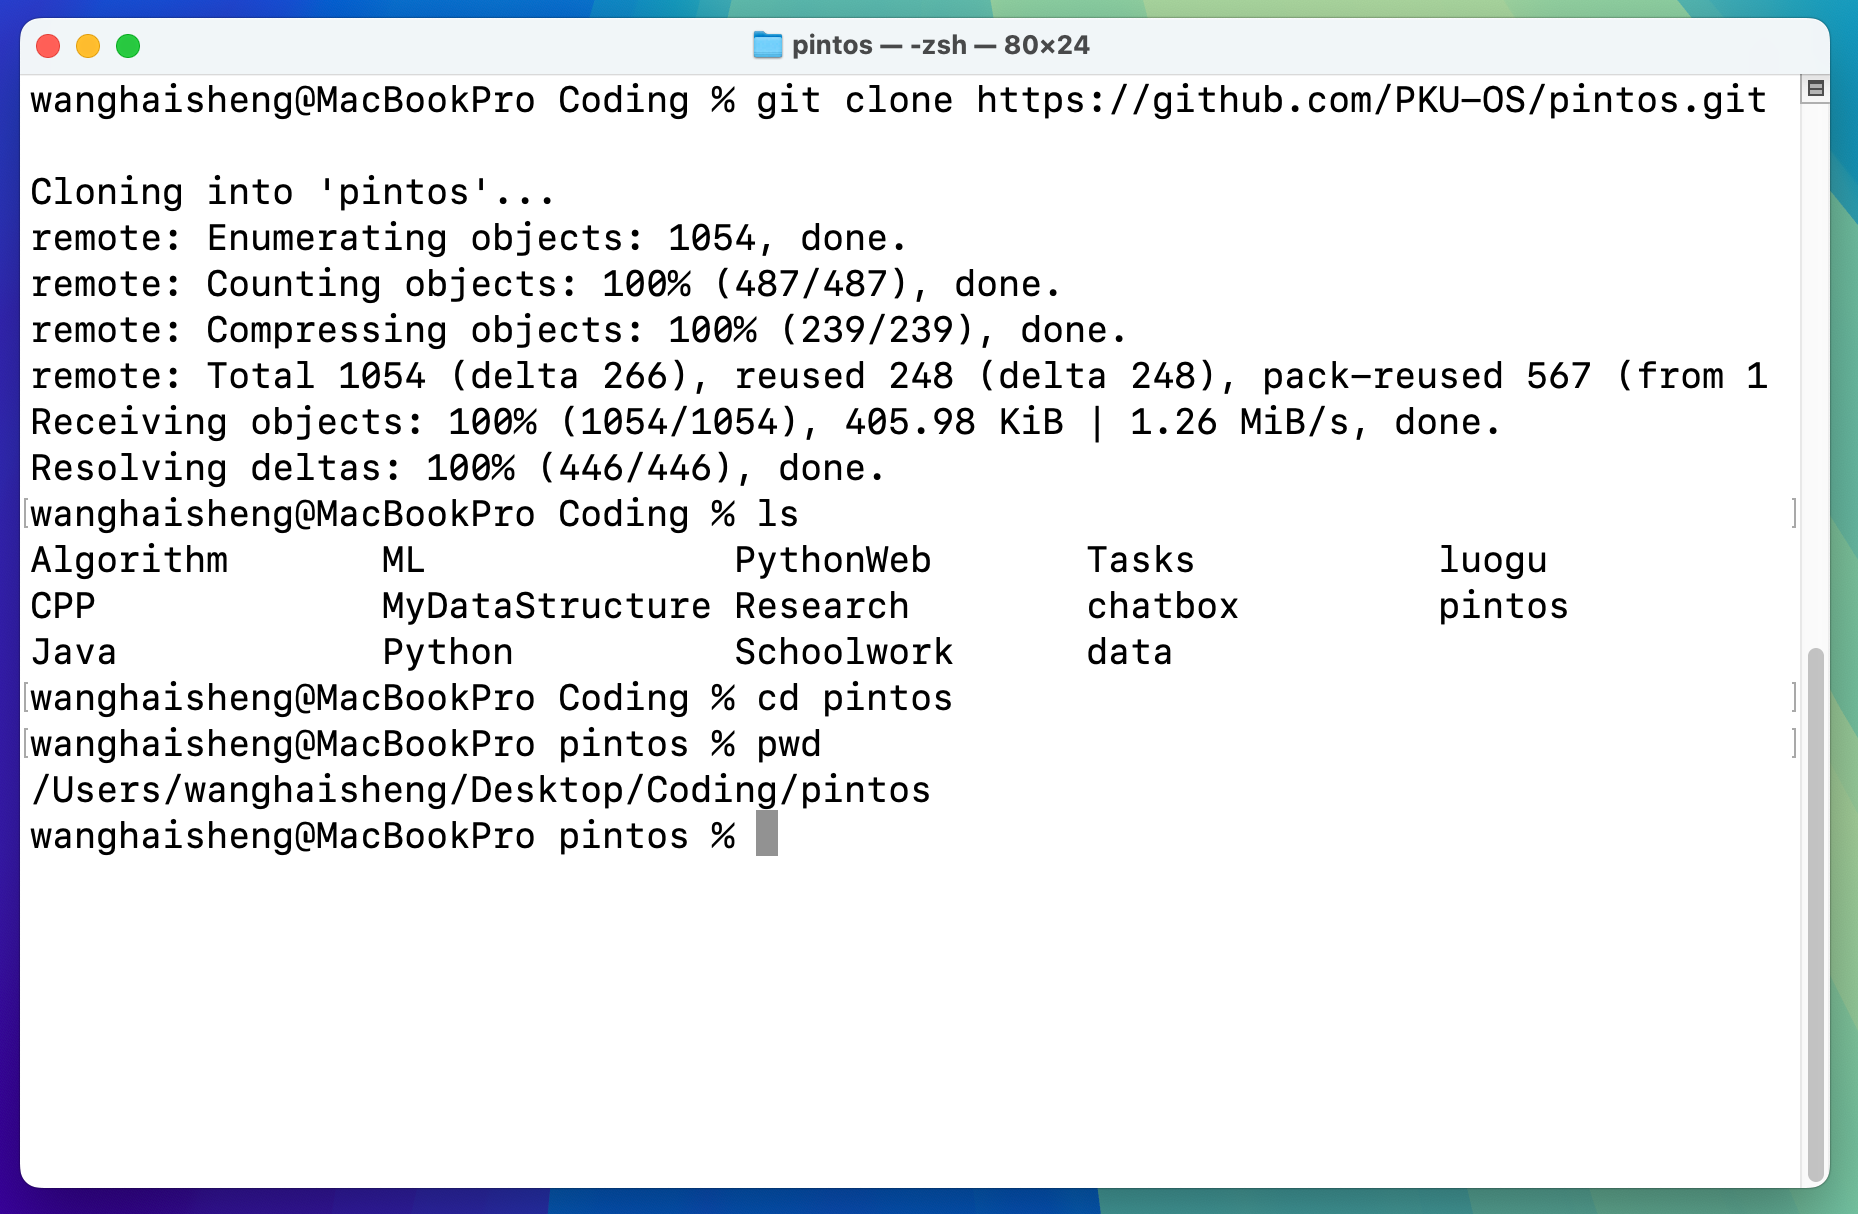
\includegraphics[width=0.9\textwidth]{img/docker_load.png}
	\caption{Docker挂载宿主系统磁盘}
\end{figure}

至此,Docker容器已经成功安装并运行PintOS,并通过文件挂载的方式管理文件。

\subsection{专用服务器}

首先,使用\texttt{git clone}命令下载PintOS源码,如下图所示。

\begin{figure}[H]
	\centering
	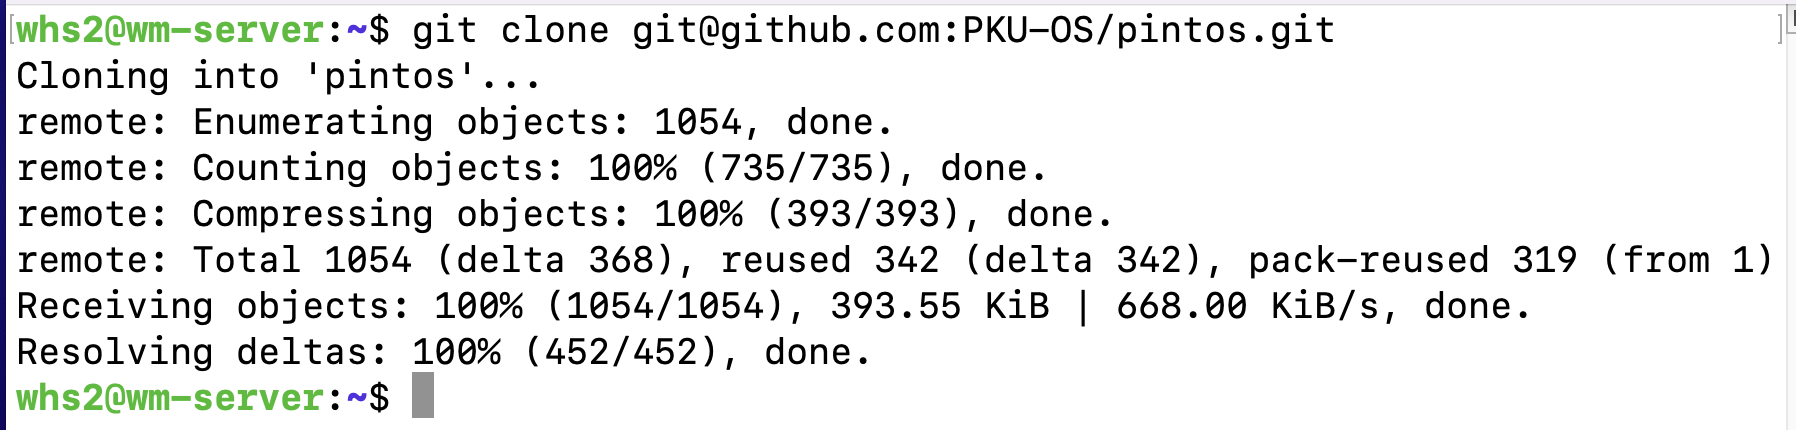
\includegraphics[width=0.9\textwidth]{img/server_git.png}
	\caption{Server下载PintOS源码}
\end{figure}

接着使用和前面类似的方法,编译PintOS源代码。至此一切正常,如下图。

\begin{figure}[H]
	\centering
	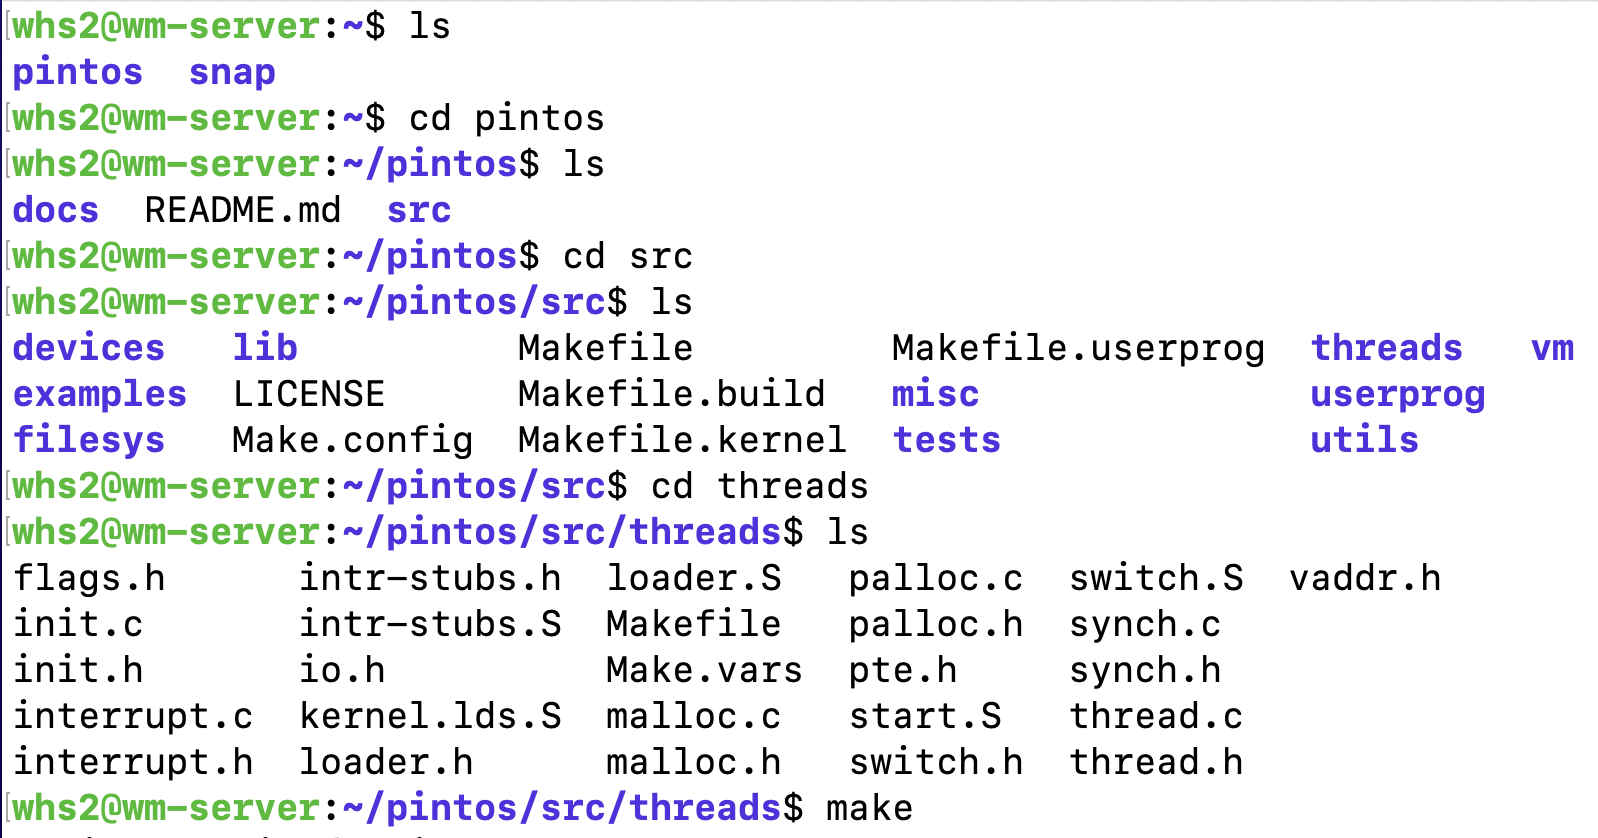
\includegraphics[width=0.9\textwidth]{img/server_make_try.png}
	\caption{Server编译PintOS源码}
\end{figure}

当输入\texttt{pintos -- -q run alarm-multiple}命令时,出现texttt{command not found}错误,如下图。

\begin{figure}[H]
	\centering
	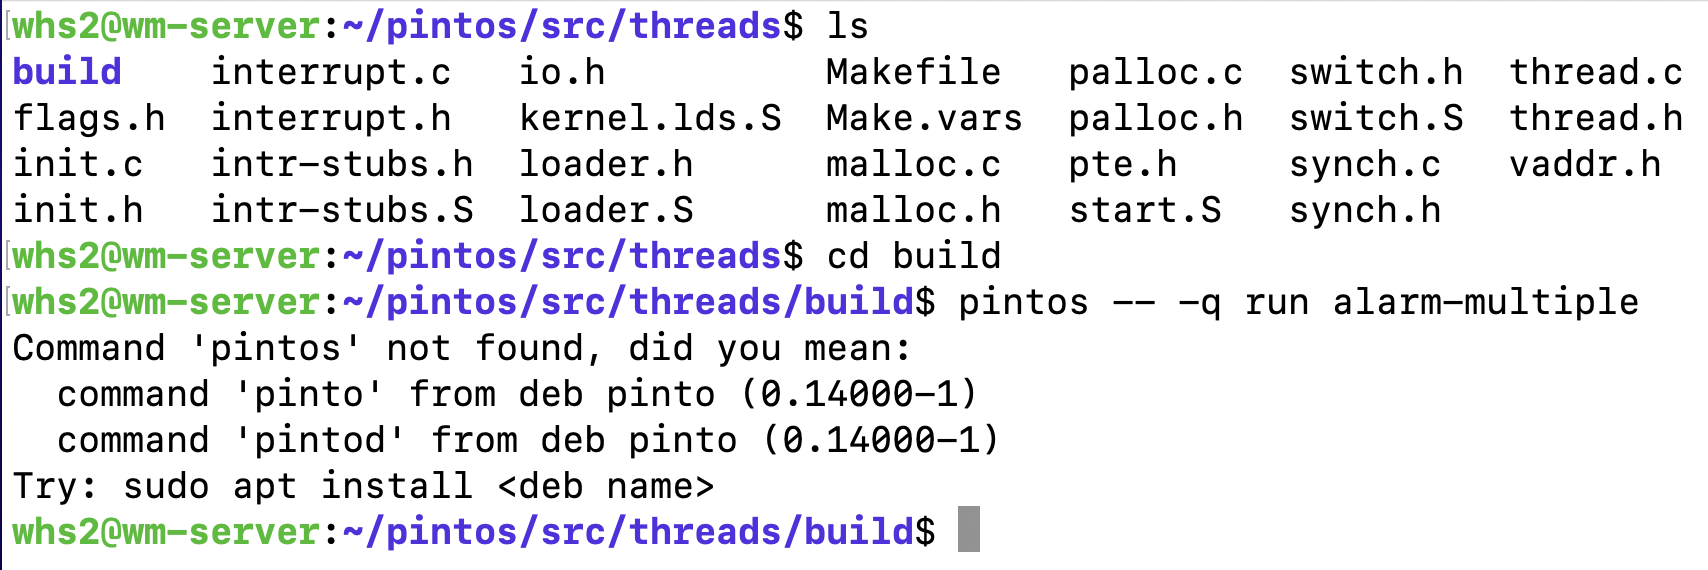
\includegraphics[width=0.9\textwidth]{img/server_command_not_found.png}
	\caption{texttt{command not found}错误}
\end{figure}

查阅资料后,发现原因是未设置环境变量。这里暂缓环境变量设置,先检查\texttt{pintos -- -q run alarm-multiple}命令是否可用。改用texttt{../../utils/pintos/ -- run alarm-multiple}命令,发现缺少\texttt{i386}支持,即32位系统支持,如下图所示。

\begin{figure}[H]
	\centering
	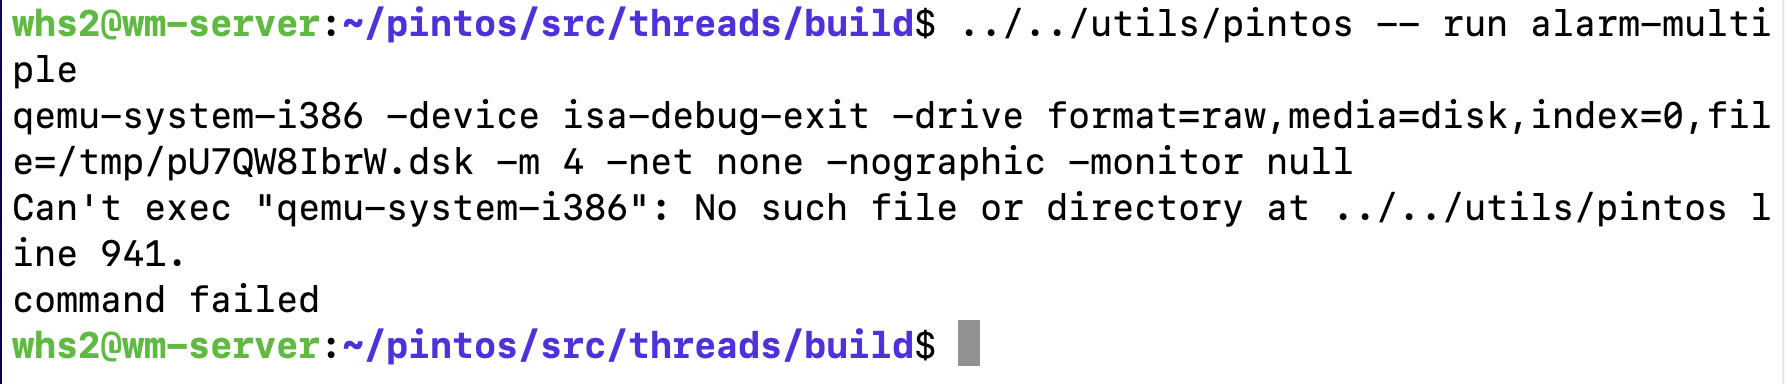
\includegraphics[width=0.9\textwidth]{img/server_failed.png}
	\caption{缺少\texttt{i386}支持}
\end{figure}

因此,根据网络教程,我开始安装Bochs模拟器。首先下载\texttt{Bochs-2.6.7},如图。

\begin{figure}[H]
	\centering
	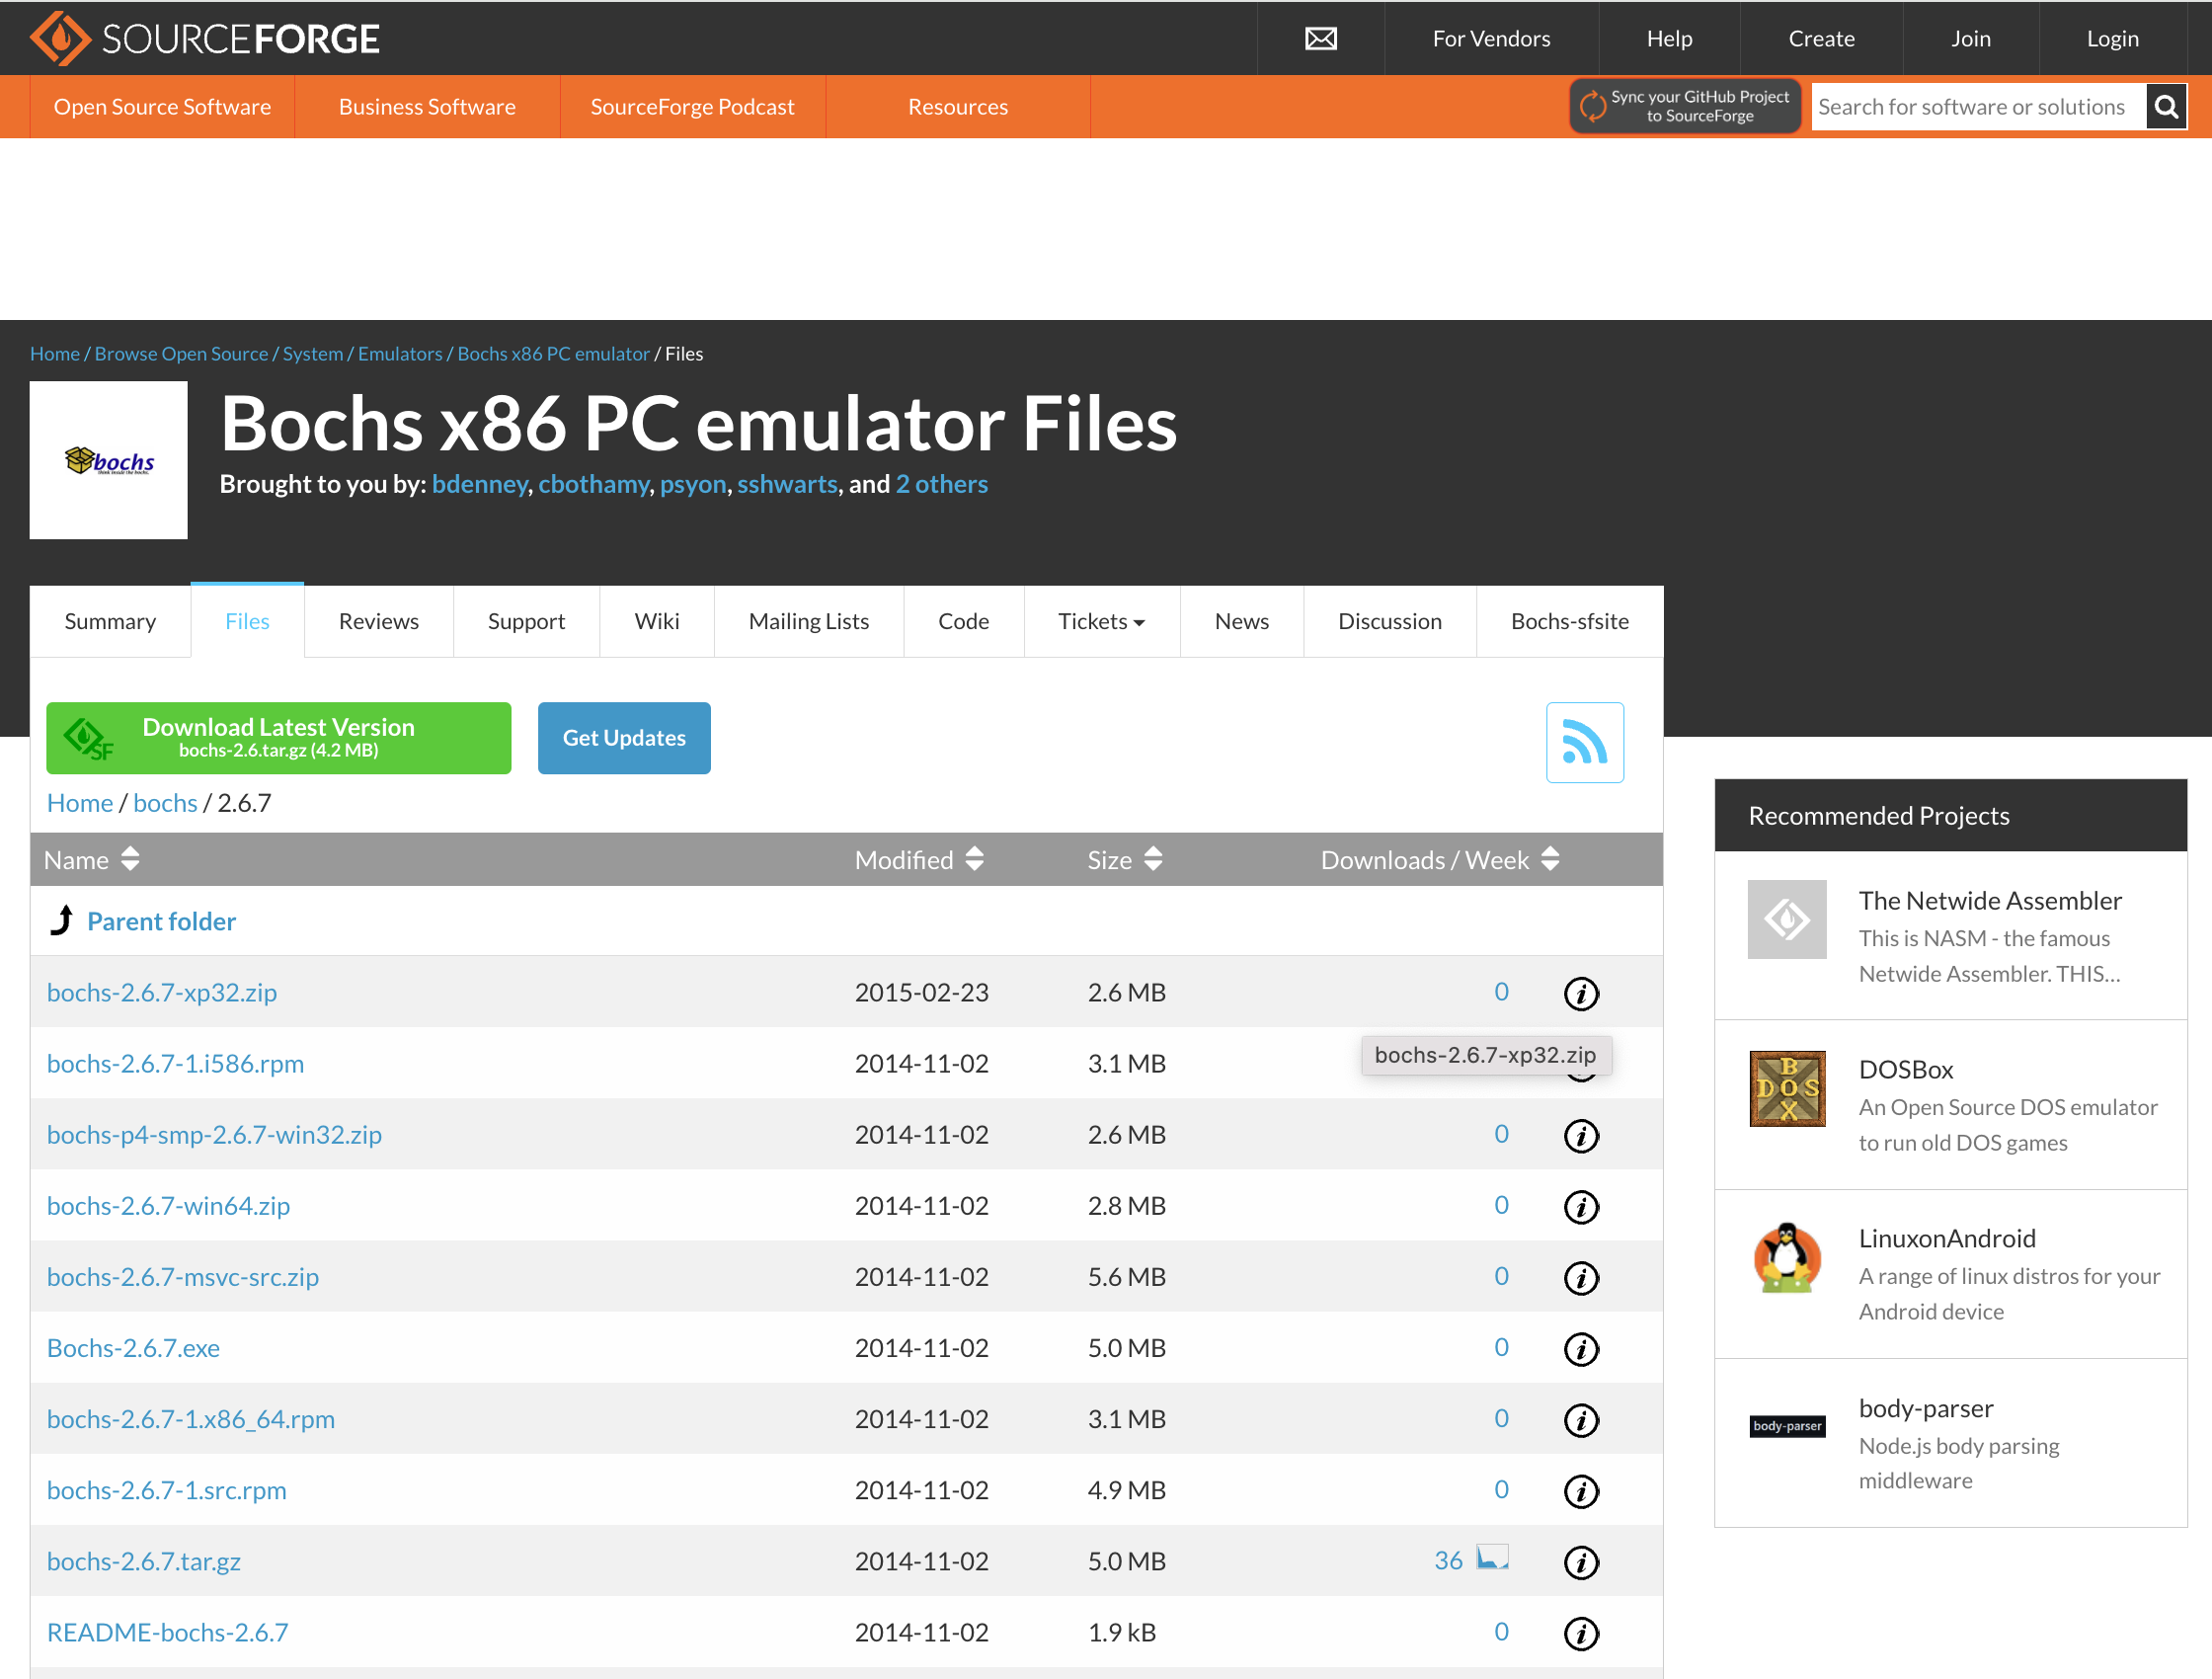
\includegraphics[width=0.9\textwidth]{img/server_bochs.png}
	\caption{下载Bochs}
\end{figure}

接着使用\texttt{scp}命令把下载好的压缩包复制到服务器上,如图。

\begin{figure}[H]
	\centering
	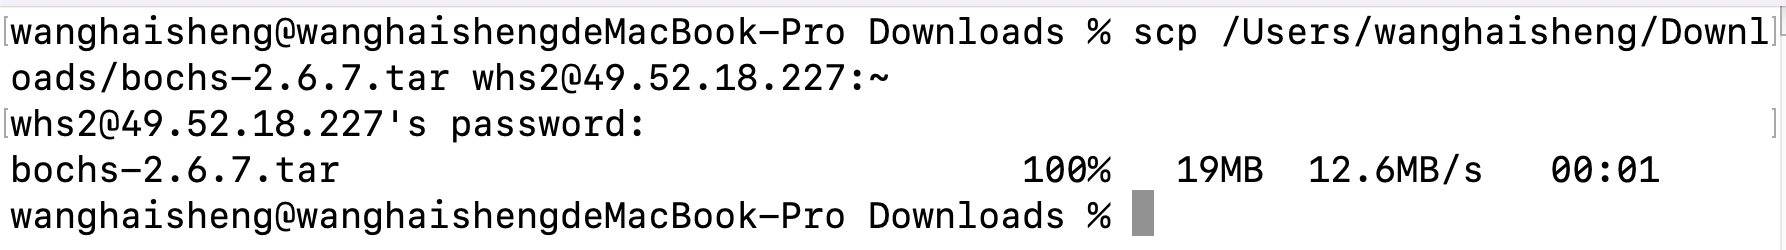
\includegraphics[width=0.9\textwidth]{img/server_bochs_scp.png}
	\caption{移动Bochs安装包至服务器}
\end{figure}

最后解压文件,完成安装,如图。

\begin{figure}[H]
	\centering
	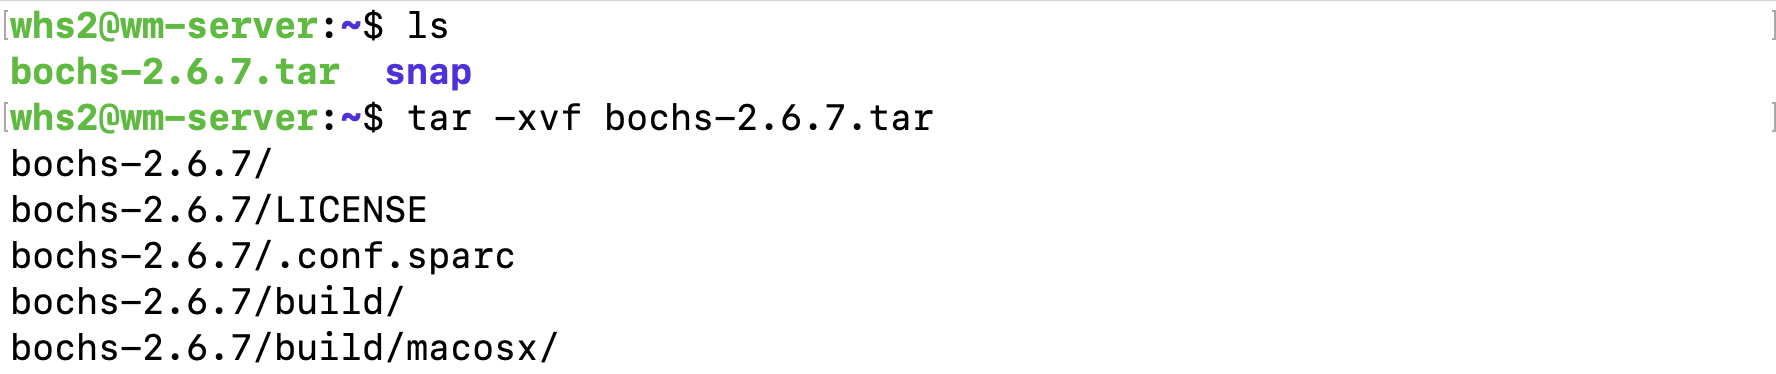
\includegraphics[width=0.9\textwidth]{img/server_bochs_install.png}
	\caption{完成Bochs的安装}
\end{figure}

在教程中,继续运行\texttt{pintos -- -q run alarm-multiple}命令即可得到最终结果。然而,在我的终端上出现了令人费解的语句,如下图所示。

\begin{figure}[H]
	\centering
	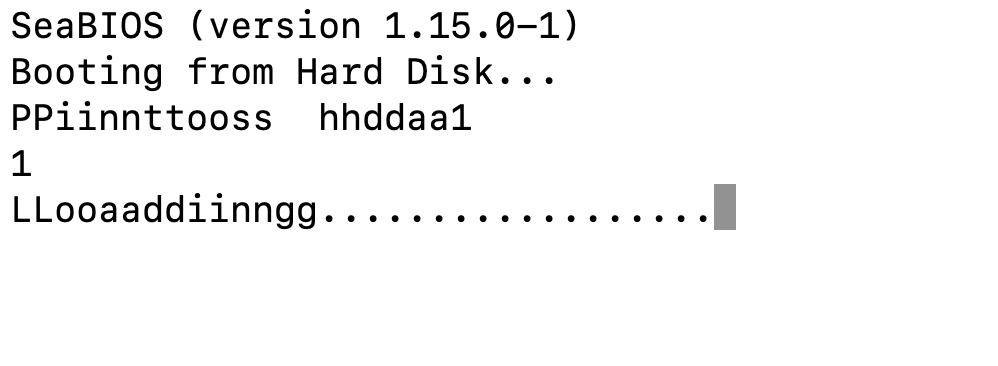
\includegraphics[width=0.6\textwidth]{img/server_error.png}
	\caption{令人费解的结果}
\end{figure}

由于缺少错误信息和日志文件,我无法弄明白到底发生了什么。在网上也没有找到类似的情况。ChatGPT给出了一种可能得原因:编译器不兼容导致文件损坏。因为网上教程使用的是更低版本的Linux系统(Ubuntu 14.04 LTS),而服务器的系统(Ubuntu 22.04 LTS)无法降级,所以实验已经无法进行下去,我不得不放弃了这PintOS种配置方法。

鉴于这一次的失败经验,我在后续WSL的安装中,都选择了较低版本的Ubuntu系统。

\subsection{Windows Subsystem for Linux (WSL)}

很遗憾,这又是一次失败的探索。前面的步骤都是一样的,但在最后一步执行\texttt{../../utils/pintos -- -q run alarm-multiple}命令时,出现了下面的错误:

\begin{figure}[H]
	\centering
	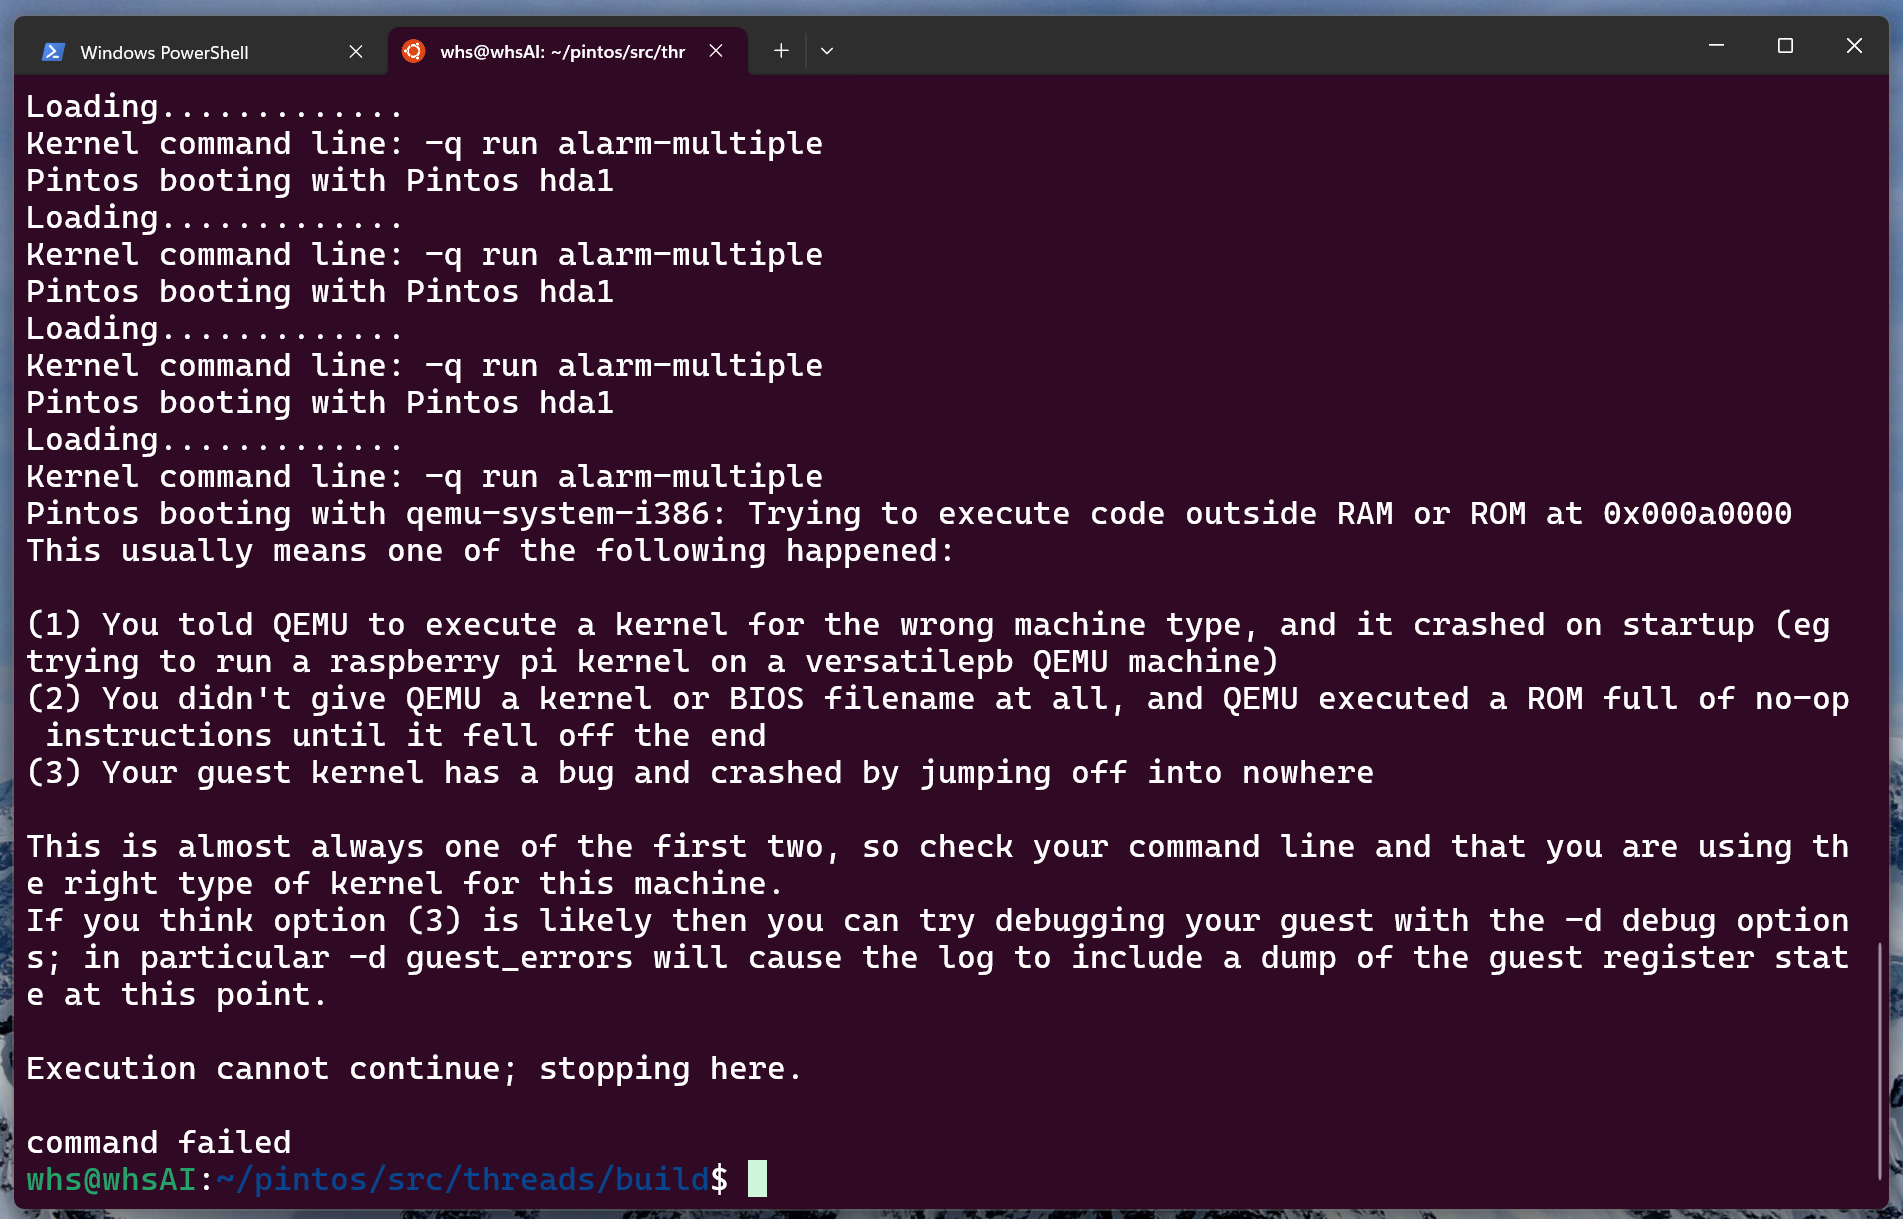
\includegraphics[width=0.9\textwidth]{img/wsl_fail.png}
	\caption{WSL内核错误}
\end{figure}

实验再一次无法进行下去,因为这个错误源自于WSL的Linux内核。简单来说,Linux内核的不完整导致Ubuntu 18.04对32位应用的支持发生兼容性错误。

具体来说,WSL2通过创建一个完整的Linux内核环境,使得Linux应用程序可以在Windows上运行。WSL2通过一种特殊的机制,使得Windows和Linux能够共享同一个文件系统。然而,由于Windows NT和Linux的权限模式不一致,当在WSL环境中混用Windows和Linux的文件系统时,可能会遇到权限冲突或不一致的问题。为了解决这个不一致问题,微软对Linux内核进行了一系列定制,从而导致了一些兼容性问题。

从本实验结果来看,WSL安装方式并不推荐。

\normalsize

\section{实验总结}

这次实验对我来说是一个浩荡的工程。与其说这是一次实验,不如说这是一次探索,一次基于纯粹热爱的探索。这次探索从四个不同的角度,让我真正走入了Linux的世界。

通过分析比较这四种安装方式,我能够在今后的学习、开发、科研中做出最合理的选择;通过研究错误信息,查询日志文件,我对编译与内核系统有了更深刻的了解;通过一次次环境的搭建,我熟悉了虚拟机、Docker、命令行、远程SSH、Git等技术。

虚拟机自不必多言,是中规中矩的稳妥选择。现代计算机速度越来越快,只要不是对显卡要求很高的领域,虚拟机都能胜任,流畅度也完全足够。在有条件的情况下,Linux服务器能提供更优秀的性能和兼容性支持。

Docker与WSL作为“不那么传统”的Linux使用方式,都有比较鲜明的优点和缺点。相比传统的虚拟机,Docker容器的理念大大降低了资源开销,强大的兼容性使其成为开发工作的首选。然而,其文件管理系统不够成熟,使用不够方便。WSL融合了Windows和Linux的文件系统,WSL2的内核也支持了绝大多数的Linux应用,是一个极具创新性的成功尝试。然而,极少数的不兼容,很有可能成为一个隐患。

这次实验给我带来的成长更在于心理上。我不再心浮气躁地看待报错,不再一看到全英文文档就嫌烦,不再照着随便找来教程生搬硬套。我沉静了下来,在图书馆一坐几个小时;遇到报错,从百度、Google、ChatGPT,到GitHub、Stack Overflow、社区文档;找了很多教程,一点点排查问题,即使失败了也一定要找到原因。

从结果来说,这次实验算不上多成功,毕竟四种方法只成功了两种。不过,实验的过程让我受益良多。希望这次实验的经历能给我的操作系统课程打下坚实的基础。

\normalsize

\end{document}